\documentclass[5p,twocolumn,10pt,times]{elsarticle}
\usepackage{amsmath}
\usepackage{hyperref}
%\modulolinenumbers[5]
\addtolength{\textheight}{8mm}
\addtolength{\textwidth}{4mm}
\addtolength{\voffset}{-10mm}
\addtolength{\hoffset}{-3mm}

\bibliographystyle{elsarticle-num-names}


% ACM template
%
%\documentclass[acmtog,anonymous,timestamp,review]{acmart}
%
%\usepackage{booktabs} % For formal tables
%




% My TK added packages and commands

	% for for using hyperref and elsarticle-num-names together in order to get \citeauthor to work
	\makeatletter
	\providecommand{\doi}[1]{%
	  \begingroup
	    \let\bibinfo\@secondoftwo
	    \urlstyle{rm}%
	    \href{http://dx.doi.org/#1}{%
	      doi:\discretionary{}{}{}%
	      \nolinkurl{#1}%
	    }%
	  \endgroup
	}
	\makeatother

	% have multiline subfigure captions be centered
	\usepackage[labelformat=parens]{subcaption} % subfigures
	\captionsetup[subfigure]{justification=centering}
	\captionsetup{subrefformat=parens} % pure refernce subfigure with parentheses: fig.10a and (b)
	%\renewcommand\thesubfigure{(\alph{subfigure})} % refernce subfigure always with parentheses: fig.10(a) and (b)

	\captionsetup[figure]{labelfont={bf},name={Fig.},labelsep=period} % use `Fig.' for figure subscript instead of `Figure'
	
	\usepackage[export]{adjustbox} % [right] alignment for includegraphics
	
	\usepackage{rotating} % turn env for rotating text in figures

	\usepackage{wrapfig} % inline figures

	% tables
	\usepackage{multirow} % multicolumn, multirow
	\usepackage{colortbl} % \cellcolor{<color>}
	\newcolumntype{C}[1]{>{\centering\arraybackslash}m{#1}}   %% centered
	\newcolumntype{R}[1]{>{\raggedleft\arraybackslash}m{#1}}  %% right aligned

	\usepackage[capitalise]{cleveref} % automatically add `Fig.'  etc before a reference.

        \usepackage{ amssymb } % \therefore
	
	\usepackage[binary-units]{siunitx} % mm and stuff
	\sisetup{per-mode = symbol}
	\DeclareSIUnit\pixel{px}

	\usepackage{units} % \nicefrac{3}{8}
	
	
	\DeclareMathOperator{\abs}{abs} % absolute function

	\usepackage[inline]{enumitem} % inline enumerate*

	\usepackage[toc,page]{appendix} % appendicces
	
	\usepackage{pgfplots}
	\usepackage{pgfplotstable} % tikzpicture table plots
	\pgfplotsset{compat=1.15}
	\usetikzlibrary{backgrounds}

	\usepackage{algpseudocode} % algorithmic
	\usepackage{algorithm} % wrapper for pseudocode to give a caption and label
	\newcommand{\pluseq}{\mathrel{+}=} %pluseq symbol

	\usepackage{listings} % for listing C++ code instead of pseudocode
	\lstset{ 
      breaklines=true,                 % sets automatic line breaking
    }

	\newcommand{\wmin}{w_\text{min}}
	\newcommand{\wmax}{w_\text{max}}
	\newcommand{\wout}{w_\text{out}}
	\newcommand{\win}{w_\text{in}}



    % \usepackage[disable]{todonotes} % notes not showed  
    % \usepackage[draft]{todonotes}   % notes showed
    \usepackage{color,soul} % caps, highlight (\hl)

    \newcommand{\todo}[1]{\hl{#1}}
    
	\newcommand{\temp}[1]{\textcolor[rgb]{0, 0, 0.2}{#1}}
	\newcommand{\tim}[1]{\temp{\todo{[Tim: #1]}}}
	\newcommand{\jun}[1]{\temp{\todo{[Jun: #1]}}}
	
	\newcommand{\old}[1]{\textcolor{gray}{#1}}

	\setulcolor{red}

	\usepackage[normalem]{ulem} % squigly underline

	\renewcommand\floatpagefraction{.8}

	% deal with missing images which are not directly included in the repo
	\iffalse
	\newcommand{\noimage}{%
	  \setlength{\fboxsep}{-\fboxrule}%
	  \fbox{\phantom{\rule{10pt}{10pt}}File missing\phantom{\rule{10pt}{10pt}}}% Framed box
	}
	\let\includegraphicsoriginal\includegraphics
	\renewcommand{\includegraphics}[2][width=\textwidth]{\IfFileExists{#2}{\includegraphicsoriginal[#1]{#2}}{\noimage}}
	\fi
% ENd of TK's added packages and commands

% ACM template
%
% Copyright
%\setcopyright{none}
%\setcopyright{acmcopyright}
%\setcopyright{acmlicensed}
%\setcopyright{rightsretained}
%\setcopyright{usgov}
%\setcopyright{usgovmixed}
%\setcopyright{cagov}
%\setcopyright{cagovmixed}
%
% DOI
%\acmDOI{10.475/123_4}
%
% ISBN
%\acmISBN{123-4567-24-567/08/06}
%
%Conference
%\acmConference[WOODSTOCK'97]{ACM Woodstock conference}{July 1997}{El  Paso, Texas USA}
%\acmYear{1997}
%\copyrightyear{2016}
%
%\acmPrice{15.00}


\begin{document}
\baselineskip11pt % SPM template

\begin{frontmatter} % SPM template

\title{A robust framework for variable extrusion width concentric toolpath generation}

%\author{Paper ID: xxx}

\author[um,tud]{Tim Kuipers}
%\author[tud]{Jun Wu}
%\author[cuhk]{Charlie Wang{\corref{cor1}}}
%\ead{cwang@mae.cuhk.edu.hk}
%\cortext[cor1]{Corresponding author}
\address[um]{Ultimaker, Utrecht, The Netherlands}
\address[tud]{Department of Design Engineering, Delft University of Technology, The Netherlands}
%\address[cuhk]{Department of Mechanical and Automation Engineering, The Chinese University of Hong Kong, Hong Kong SAR, China}


\begin{abstract}
abstract
\end{abstract}

%
% The code below should be generated by the tool at
% http://dl.acm.org/ccs.cfm
% Please copy and paste the code instead of the example below.
%
%\begin{CCSXML}
%\end{CCSXML}

%\ccsdesc[500]{Computer systems organization~Embedded systems}
%\ccsdesc[300]{Computer systems organization~Redundancy}
%\ccsdesc{Computer systems organization~Robotics}
%\ccsdesc[100]{Networks~Network reliability}

%\keywords{Space-filling Curve, Fractal, Dithering} % ACM
\begin{keyword} % SPM
keyword
\end{keyword}

\end{frontmatter}




 \temp{%Table of contents just for reviewing purposes
 \tableofcontents
 }

\section{Introduction}
3D printing enables the fabrication of complex geometry under few design constraints compared to conventional fabrication techniques.
Recent developments have seen a rapid growth in both the use and capabilities of desktop 3D printing systems.
%The rapid spread of 3D printing through different industries and types of application calls for the possibility to manufacture a wide range of geometries while guaranteeing mechanical properties of the resulting parts.
Fused Deposition Modeling (FDM) is one of the most common 3D printing techniques.
It is widely used because of the versatility in the types of plastic which can be used and the relatively low running costs.
FDM printers are used, for example, in showcasing scale models of buildings, casings for electronics, prototypes for blow molded parts, jigs and fixtures.
Recent research developments have investigated manufacturing complex volumetric structures such as microstructures~\cite{bates2018compressive,Al-Ketan2018,Maskery2018} and topology optimized structures~\cite{Zegard2016SMO,Wu2019a,Cheng2019}.
Many of these applications involve 3D models with detailed features within the order of magnitude of the printing resolution, which restrains the field of the process planning algorithms.

FDM printers extrude semi-continuous beads of molten plastic through a nozzle, which moves along a planned toolpath within each layer of a 3D object.
A common strategy to accurately manufacture a given 3D model is to extrude along a contour-following path,
because the position and shape of the toolpath can be controlled relatively accurately.
Filling up a shape using parallel straight lines would expose defects of the size of the hole in the nozzle, which is generally an order of magnitude larger than the resolution of the positioning system.
Contour-parallel extrusion therefore leads to a less bumpy outline shape than direction-parallel extrusion does.


The simple technique for generating the dense contour-parallel toolpaths of a layer consists in performing uniform inward offsets with the size of the nozzle from the outline shape.
However, for geometrical features which are not an exact multiple of the nozzle size this method produces areas where an extrusion bead is placed twice: \emph{overfill} areas; and areas which are not filled at all: \emph{underfill} areas.
See \cref{intro_wedge_uniform}.
Overfills cause a buildup of pressure in the mechanical extrusion system, which can result in bulges or even a full print failure.
Underfills on the other hand, can cause a drastic decrease in the part stiffness or even for small features not to be printed at all.
These problems are exacerbated for models with layer outlines with small features, because the over- and underfill areas are relatively large compared to the whole part.

One promising direction to avoid over- and underfills is to employ toolpath with adaptive width.
\citeauthor{Ding2016a} developed a toolpath strategy for wire and arc additive manufacturing which produces a width variation typically lower than a factor of $3$, but is sometimes far greater~\cite{Ding2016a,Xiong2019}.
However, the range of widths manufacturable by FDM systems is limited.
A nozzle of \SI{0.4}{\milli\meter} will typically start to cause fluttered extrusion around lines narrower than \SI{0.3}{\milli\meter} and lines will start to bulge upward if they are wider than the flat part of the nozzle, which is typically \SI{1.0}{\milli\meter}.
%Therefore, a limited range of widths is required by the hardware system.

The current state-of-the-art for FDM printing developed by \citeauthor{Jin2017JMS} employs a strategy which alters the widths of the centermost beads at most by a factor of $2$~\cite{Jin2017JMS},
which is similar to the strategy employed by the open source industry standard software package Ultimaker Cura~\cite{cura}.
See \cref{intro_wedge_centered}.
Still, controlling the extrusion width through movement speed changes or through volumetric flow control (e.g. linear advance) yields diminishing accuracy for deposition widths farther away from the nozzle size,
since process parameters such as nozzle temperature are optimized for beads with the nozzle size.
Moreover, reducing the variation in width is beneficial for limiting the variation in mechanical properties of the resulting product, meaning it conforms better to a simulation which employs a homogeneity assumption.
Therefore, a narrower range of widths is desirable.

In this paper we propose a framework for planning toolpaths with control over the adaptive width for minimizing over- and underfill. 
We show that this framework supports various control schemes for determining the bead spacing and extrusion widths. 
For FDM printing in particular we propose a novel scheme which reduces the amount of over- and underfill while ensuring the extrusion beads deviate little from the nozzle size.
See \cref{intro_wedge_distributed}. 
% In order to avoid over- and underfills in regions which are not as wide as an exact multiple of the nozzle size we need algorithms which produce toolpaths which employ adaptive bead width.
% Some such toolpath generation techniques have already been developed.


\begin{figure}\centering
\setlength{\figwidth}{.9\columnwidth}
\setlength{\figwidthTwo}{.05\columnwidth}
\begin{subfigure}{\figwidth}\centering
\parbox[b]{\figwidthTwo}{\subcaption{}\label{intro_wedge_uniform}}
\includegraphics[width=\figwidth]{sources-intro-TEST-naive-accuracy.png}
\end{subfigure}
\begin{subfigure}{\figwidth}\centering
\parbox[b]{\figwidthTwo}{\subcaption{}\label{intro_wedge_centered}}
\includegraphics[width=\figwidth]{sources-intro-TEST-Center-widths.png}
\end{subfigure}
\begin{subfigure}{\figwidth}\centering
\parbox[b]{\figwidthTwo}{\subcaption{}\label{intro_wedge_distributed}}
\includegraphics[width=\figwidth]{sources-intro-TEST-InwardDistributed-widths.png}
\end{subfigure}
\caption{
Illustration of different toolpath for a wedge shape.
\subref{intro_wedge_uniform} Toolpath using uniform offsetting results in large overfill (orange) and underfill (azure).
\subref{intro_wedge_centered} Toolpath with adaptive width~\cite{Jin2017JMS} where beads that are wider or narrower than the nozzle size are indicatd in red and blue, respectively.
\subref{intro_wedge_distributed} Our approach minimizes over- and underfill with beads close to the nozzle size.
}
\label{intro_wedge}
\end{figure}


Our contributions are as follows:
\begin{itemize}
\item A geometric framework for generating densely filling contour-parallel toolpaths employing adaptive width, according to any beading scheme which decides on the bead spacing and widths.
\item A specific beading scheme for FDM printing which reduces the amount of deviation in the extrusion widths, and which promotes smooth toolpaths that are equal to the preferred width toward the outline of the shape.
\end{itemize}



%This work is patent pending, but the source code is available open source.



\section{Related Work}

Given a planar contour, representing the intersection of a plane and a 3D solid object, the task is to generate a path in the domain bounded by the contour.
The nozzle is then instructed to move along the path while extruding material.
The deposited material covers the path with a certain width.
Toolpath generation is an integral part of process planning for 3D printing.
For an overview of the processing pipeline, we refer to the survey by \citeauthor{Livesu2017CGF}.~\cite{Livesu2017CGF} .
For reducing printing time and material cost, sparse infill structures such as triangular and hexagonal patterns have been used to approximate the interior of 3D shapes.
In this paper, we focus on generating toolpath that seamlessly covers the entire 2D contour.
This is sometimes called dense infill~\cite{Livesu2017CGF}.

Toolpath has a direct influence on the printing time, material cost, and mechanical properties of the printed object.
There are a few desirable properties for the toolpath.
First, the path shall be as continuous as possible.
A discontinuous path requires to stop and restart material extrusion. 
For certain material such as TPU, this could lead to material defect~\cite{KUIPERS2019CAD}.
Furthermore, a smooth path is often preferred.
A path with a lot of sharp turns requires to slow down the movement of the nozzle, and this consequently prolongs the printing process.
Second, the path, extended with a certain width, ideally shall cover the bounded region no voids or gaps --  underfilling, and no overlap -- overfilling.
Our method is primarily concerned with this requirement. 

Direction parallel and contour parallel are two basic toolpath strategies.
Direction parallel (or zig-zag) toolpath fills an arbitrarily shaped contour with a set of parallel, equally spaced line segments.
These parallel segments are linked at one of their extremities, to avoid frequent stop and restart.
Contour parallel toolpath typically consists of a set of equally spaced offset contours from the slice boundary.
A strategy to connect the parallel offsets was introduced in~\cite{KUIPERS2019CAD}.
One of the problems with contour parallel toolpath is that it tends to leave gaps within the slices.
This is due to the fact that the offset contour meets around the medial axis and the remaining space might not match exactly the (constant) deposition width.
To avoid problems with such gaps, hybrid approaches that combine direction and contour parallel are often used~\cite{Mcmains2000DETC,Jin2013adaptive}.
Close to the slice boundary there are a few contour parallel curves, while in the interior there is a zig-zag pattern.
For complex shapes, the entire cross-section could be decomposed into a set of patches, and for each of them, the basic strategies can be applied~\cite{Ding2014}.
To reduce the number of sharp turns thereby enable faster motions, \citeauthor{Zhao2016} proposed to use Fermat spiral to cover the contour ~\cite{Zhao2016}.
Alternative toolpath patterns, seen also in CNC machining, include space-filling curves~\cite{Cox1994CAD,Griffiths1994,Shaikh2016}.

Our idea to reduce under- and over-filling is to deposit material with a varying width.
This allows the opportunity to locally match the nonuniform space between adjacent paths, and thus to ensure a better coverage of the domain.
Material extraction with a varying width can be realized by changing the extrusion rate or the nozzle travel velocity~\cite{Ertay2018}.
However, we note that the range of possible widths is not unlimited.
For instance, printing a width that is twice the nozzle radius is challenging.
Our method to reduce underfilling is related to the work by \citeauthor{kao1998optimal}~\cite{kao1998optimal}.
Instead of uniform offsetting, they produced adaptive offsetting toolpaths based on the geometry skeleton.
This approach originally handles simply geometry where there are no branches in the medial axis.
This was extended by \citeauthor{Ding2016a} to handle complex shapes~\cite{Ding2016a}.
For this purpose, they made use of the medial axis to decompose the slice into a set of simple geometries.
This extension, however, inherits a problem in the original method.
From any point in the geometry skeleton to the boundary, the number of contours is constant.
Since the distance may vary considerably, this strategy leads to a toolpath with widths that may differ by a factor of two or more.
In this paper we propose an adaptive beading strategy to address this problem.

Besides under- and over-filling, there are a few other robustness issues in toolpath generation, especially concerning thin geometric features.
\citeauthor{Moesen2011} proposed a method to make beam compensation more reliable for thin geometric features~\cite{Moesen2011}.
\citeauthor{Behandish2019a} presented a method to characterize local- topological discrepancies due to material under- and over-deposition, and used this information to modify the as-manufactured outcomes~\cite{Behandish2019a}.




% \subsection{Toolpath strategies}
% Simple Zig-Zag toolpathing strategy. \cite{mcmains2000layered}
% Patchwise Zig-Zag toolpathing strategy. \cite{Ding2014}

% Combining concentric toolpaths into continuous extrusion spirals. \cite{Held2009}

% Fractal based toolpaths. \cite{Griffiths1994, mandal2016}

% \subsection{Space filling toolpaths}
% \todo{find other literature which tries to minimize underfilling and overfilling which is not based on a skeletonization.}


% \subsection{Medial axis based toolpaths}
% Adjusted Medial Axis Transform (MAT) structure for only printing the outer wall, rest area to be filled using normal infill. \cite{Moesen2011}
% \Cref{moessen}
% Problem: small grey areas which are too small for the second wall lines.

% Figuring out underfilling and overfilling arteas in concentric fill and using single squigly lines to prevent overfilling. \cite{Jin2017}
% \Cref{jin}

% Using variable width lines to fit a precise amount of lines using the MAT.
% \cite{Ding2016a} apply the method from \cite{kao1998optimal}.
% \Cref{ding}

% \begin{figure}
% \begin{subfigure}{0.45\columnwidth}
% 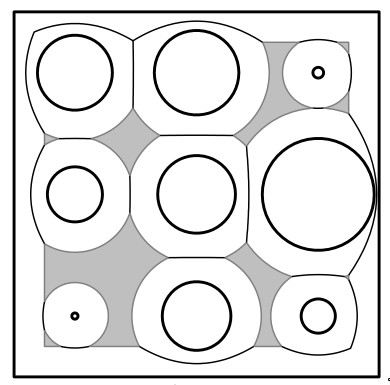
\includegraphics[width=\columnwidth]{sources/related_work/moessen.jpg}
% \caption{\citeauthor{Moesen2011}}
% \label{moessen}
% \end{subfigure}
% \begin{subfigure}{0.45\columnwidth}
% 
\includegraphics[width=\columnwidth]{sources/related_work/jin.jpg}
% \caption{\citeauthor{Jin2017}}
% \label{jin}
% \end{subfigure}
% \end{figure}

% \begin{figure}
% \centering
% 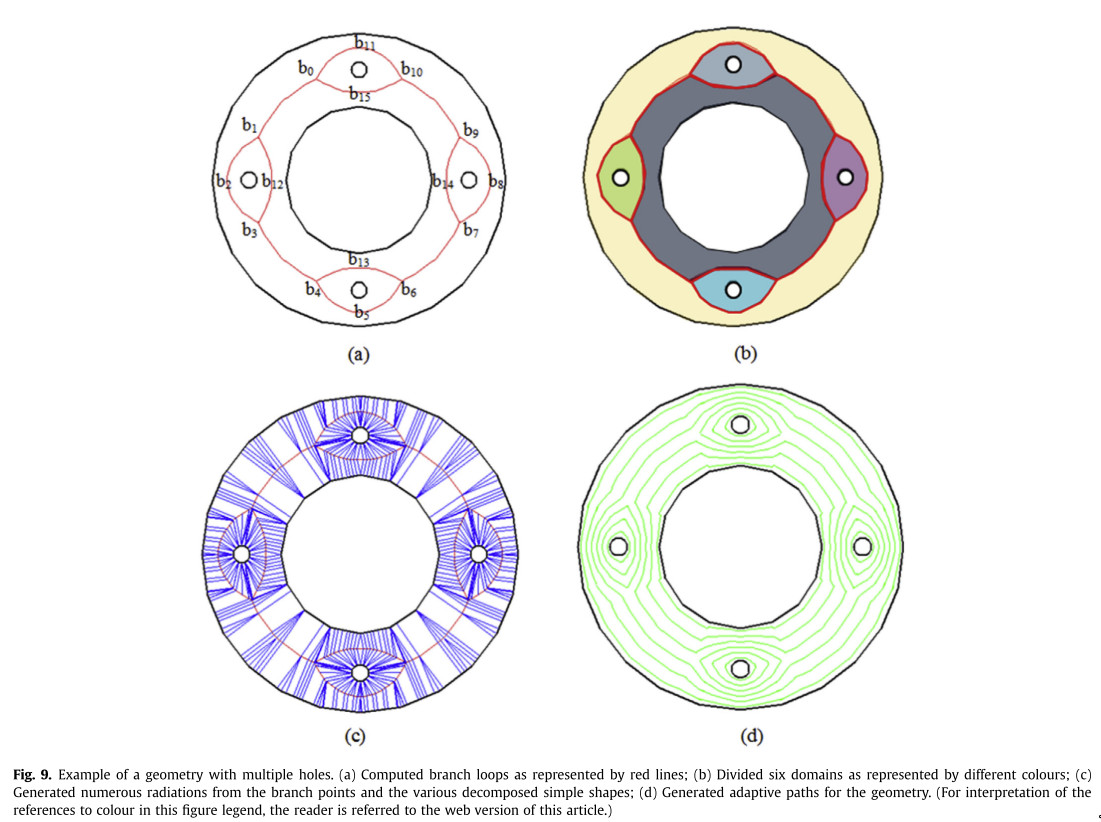
\includegraphics[width=\columnwidth]{sources/related_work/ding.jpg}
% 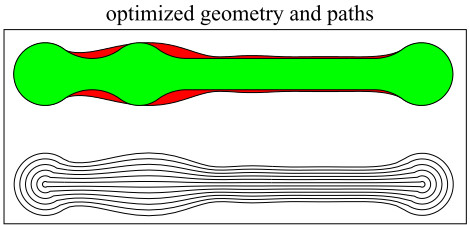
\includegraphics[width=.7\columnwidth]{sources/related_work/kao.jpg}
% \caption{Path planning strategies proposed by Kao (bottom) and employed in FDM by Ding et al (top).}
% \label{ding}
% \end{figure}

% \subsection{Variable extrusion width}

% Changing extrusion rate and temperature to match a given velocity. \cite{Ertay2018}

% Changing velocity in order to change extrusion rate.
% Shortly discussed in \cite{Kuipers2018}.
% \todo{find another reference}

\section{Method}
\subsection{Overview}

Given arbitrarily shaped polygons which represent the 2D outline of a layer of a 3D model, our method generates extrusion toolpaths with varying width, i.e. a set of polylines where each site consists of a location and an extrusion width;
in between the sites we linearly interpolate the position and extrusion width.

Our method starts with computing the skeleton of the input polygon based on the medial axis transform (MAT), a strategy that has been commonly used for generating contour parallel toolpaths~\cite{eiamsa2003toward}. 
We visualize the skeleton as the union of cones (UoC) (\cref{sec_surface_construction}), by raising each point in the domain to a height that equals the shortest distance from the point to the polygon boundary (\cref{overview_uoc}).
Contour parallel toolpath with uniform width can be interpreted as the intersection of the union of cones with a set of planar planes at equally spaced heights (\cref{3d_surface_overview}\subref{overview_outline}-\subref{overview_uniform_paths}).

As depicted in \cref{3d_surface_overview_center}, our method first identifies edges and nodes in the skeleton that are located in the center of the polygon, which correspond to ridges and peaks in the UoC  (\cref{sec_center_classification}).
The heights $\tilde{b}$ at these elements are then quantized to an integer number of beads $\bar{b}$.
To ensure a smooth toolpath between regions with quantized integer heights that differ, we add new nodes in the skeleton with quantized heights and interpolate the heights $\hat{b}$ in between (\cref{sec_central_height_adjustment}).
The union of cones corresponding to the smoothed skeleton is then sliced at regular intervals to obtain toolpaths with varying spacing, which translates into varying width (\cref{sec_toolpath_extraction}).

% We describe how to construct the mesh of the UoC in \cref{sec_surface_construction} and
% explain how to identify central regions in \cref{sec_center_classification}.
% Quantizing and smoothing the heights in the central mesh regions are handled in \cref{sec_central_height_adjustment}.
% We then describe how to deal with heights in the periphery in \cref{sec_peripheral_height_adjustment}
% and describe the toolpath extraction algorithm in \cref{sec_toolpath_extraction}.

This section explains how we generate toolpaths using our framework with uniform bead widths and evenly distributed locations between the center of the polygon and the outline.
In \cref{sec_generalization} we describe how to apply the framework to different beading schemes and we show several such beading schemes.


% The simple technique consists of consecutive inward offsets from the outline using a uniform bead width.
% These offsets can be generated from the medial axis transform (MAT).
% The medial axis transform can be conceptualized as the skeleton of the mesh of the volume defined by the union of all cones (with the same incline) which are touching the input shape~\cite{blum1967transformation}.
% The constant width insets are the intersections between the Union of Cones (UoC) and horizontal planes at regular intervals.
% We can therefore use the MAT to efficiently calculate the consecutive offsets which define the uniform toolpathing~\cite{eiamsa2003toward}.

% For the uniform offsetting technique the overfill and underfill problems arise in the center,
% because constant widths inward steps might not resolve to the arbitrary diameter of the outline shape.
% Our framework can be seen as a way to change the mesh of the UoC such that the heights at the center are aligned with the slicing planes.

% Our framework can be thought of as following these steps:
% \begin{itemize}
% \item Compute the skeleton of the input shape
% \item Assign each node a height in terms of bead count based on the local feature size
% \item Identify central regions of the UoC
% \item Quantize the height of central ridges and peaks
% \item Smooth out sharp transitions between regions with different integer heights
% \item Determine the heights in the periphery (non-central regions)
% \item Slice the mesh at regular intervals to get the toolpaths to fill the input shape
% \end{itemize}
% See \cref{3d_surface_overview}.






\begin{figure*}
\centering
\setlength{\figheight}{.15\textwidth}
\setlength{\figwidth}{.15\textwidth}
\setlength{\figwidthTwo}{.22\textwidth}
\begin{subfigure}{\figwidth}\centering
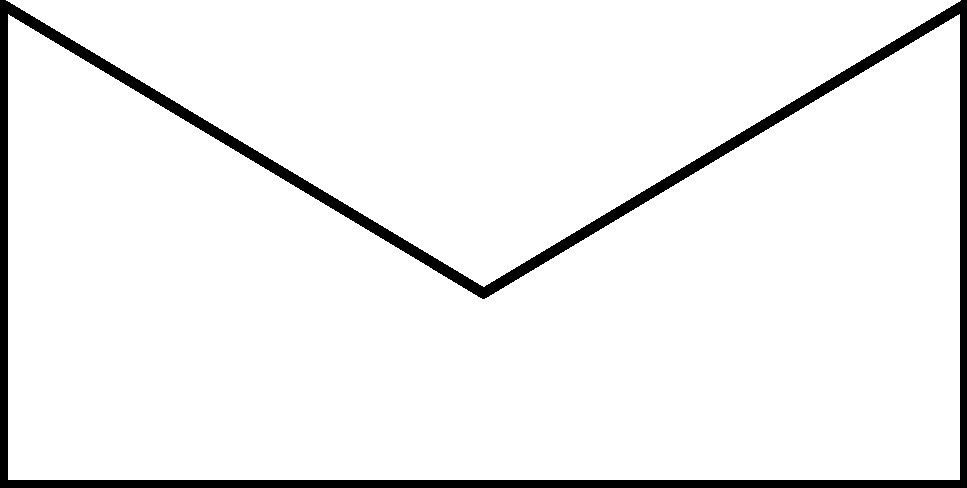
\includegraphics[width=\figheight,rotate=-90]{sources/method/overview/2D/input.pdf}
\caption{Layer outline}\label{overview_outline}
\end{subfigure}
\begin{subfigure}{\figwidth}\centering
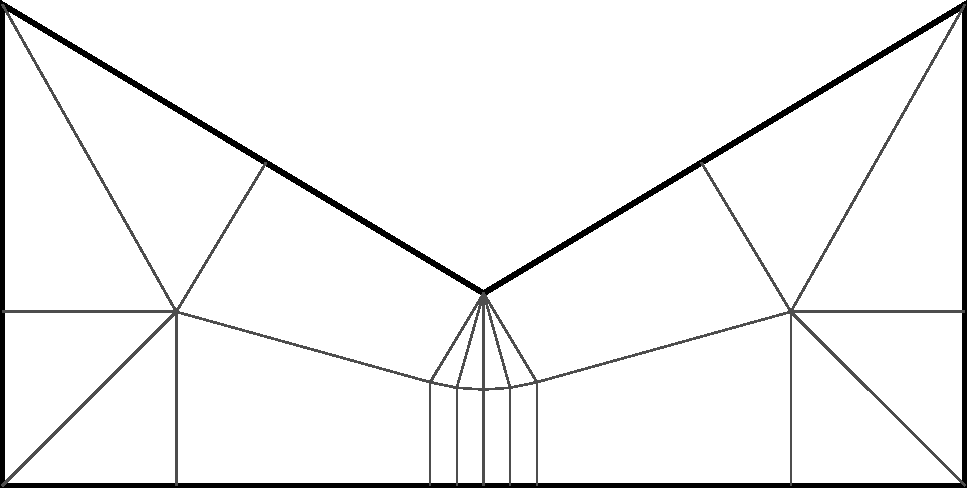
\includegraphics[width=\figheight,rotate=-90]{sources/method/overview/2D/uoc.pdf}
\caption{Skeleton}\label{overview_skeleton}
\end{subfigure}
\begin{subfigure}{\figwidthTwo}\centering
\hspace*{\tempheightTwo}
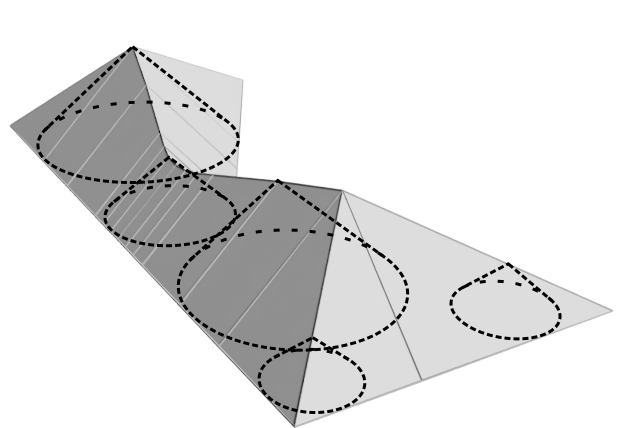
\includegraphics[height=\figheight]{sources/method/overview/surface/UoC_with_cones.png}
\caption{Union of cones}\label{overview_uoc}
\end{subfigure}
\begin{subfigure}{\figwidthTwo}\centering
\hspace*{\tempheightTwo}
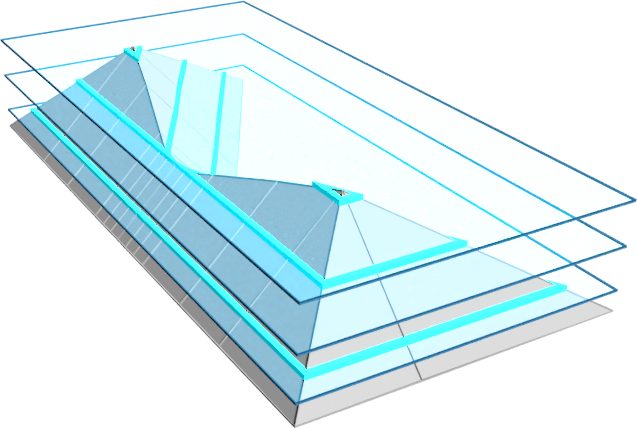
\includegraphics[height=\figheight]{sources/method/overview/surface/sliced_naive_cropped.png}
\caption{Slicing}\label{overview_uniform_sliced}
\end{subfigure}
\begin{subfigure}{\figwidth}\centering

\includegraphics[width=\figheight,rotate=-90]{sources/method/overview/2D/naive.png}
\caption{Uniform paths}\label{overview_uniform_paths}
\end{subfigure}


\setlength{\figwidth}{.22\textwidth}
\setlength{\figwidthTwo}{.17\textwidth}
\setlength{\figwidthTree}{.22\textwidth}
\setlength{\tempheight}{-0.3cm}
\setlength{\tempheightTwo}{-0.5cm}
\begin{subfigure}{\figwidth}\centering
\hspace*{\tempheightTwo}
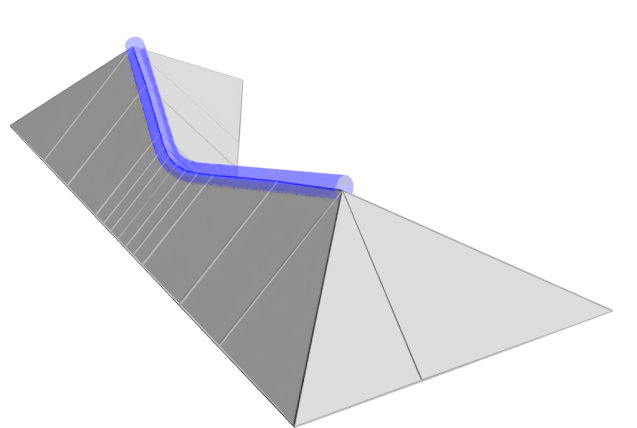
\includegraphics[height=\figheight]{sources/method/overview/surface/marking_cropped.png}

\vspace{\tempheight}

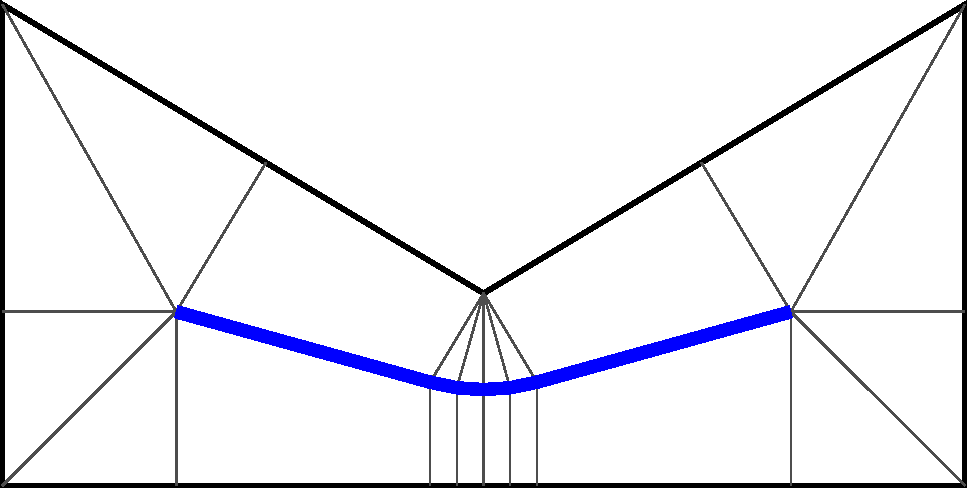
\includegraphics[width=\figheight]{sources/method/overview/2D/marked.pdf}
\caption{Center identification}\label{3d_surface_overview_center}
\end{subfigure}
\begin{subfigure}{\figwidth}\centering
\hspace*{\tempheightTwo}
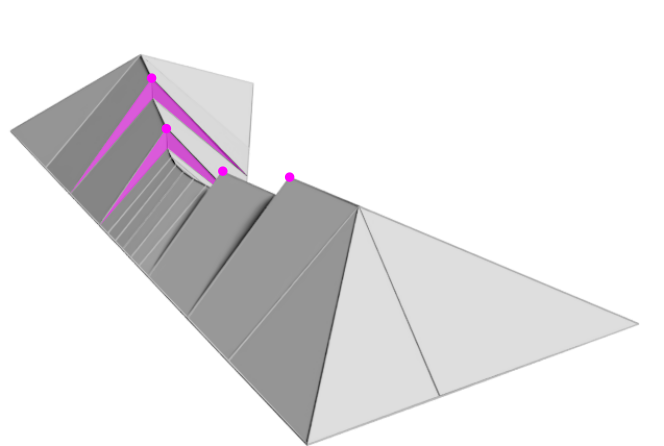
\includegraphics[height=\figheight]{sources/method/overview/surface/quantized.png}

\vspace{\tempheight}

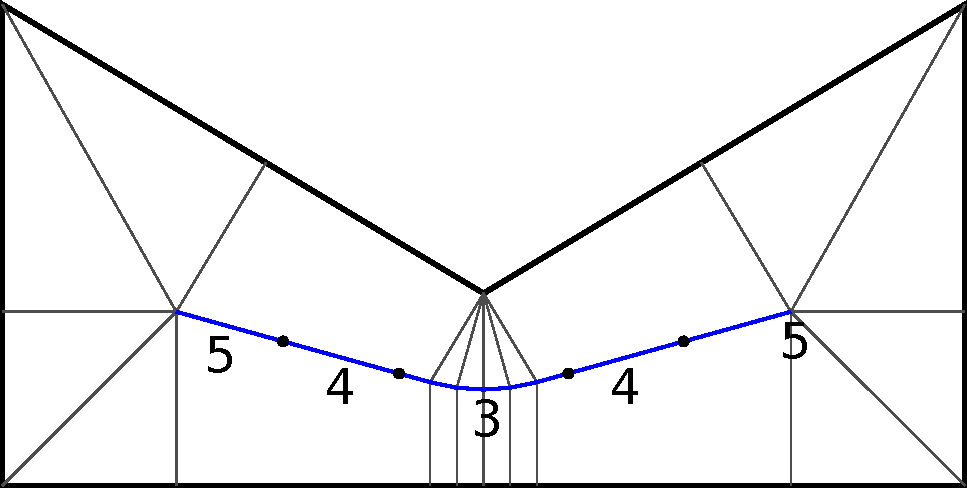
\includegraphics[width=\figheight]{sources/method/overview/2D/rounded.pdf}
\caption{Quantization}\label{3d_surface_overview_rounded}
\end{subfigure}
\begin{subfigure}{\figwidth}\centering
\hspace*{\tempheightTwo}
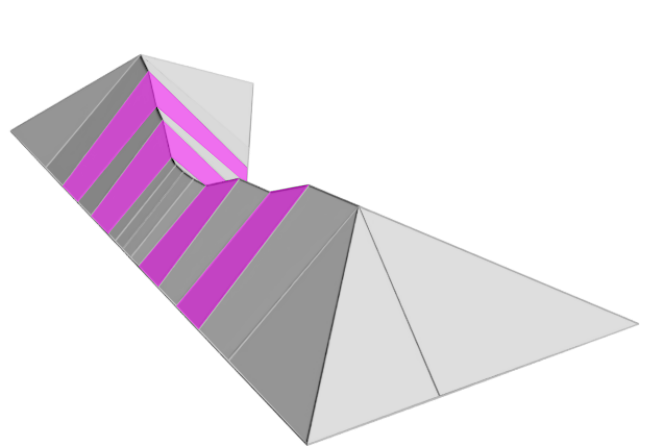
\includegraphics[height=\figheight]{sources/method/overview/surface/smoothed_magenta.png}

\vspace{\tempheight}

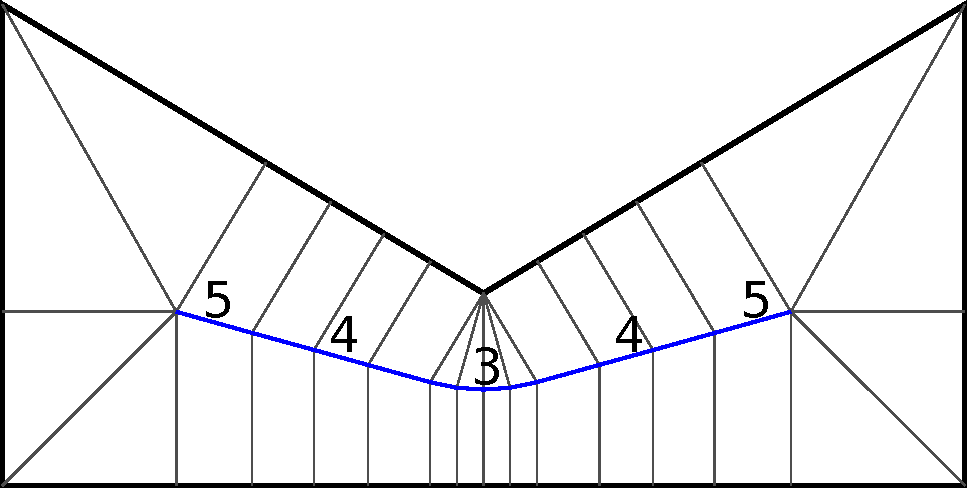
\includegraphics[width=\figheight]{sources/method/overview/2D/smoothed.pdf}
\caption{Smoothing}\label{3d_surface_overview_smoothed}
\end{subfigure}
\begin{subfigure}{\figwidth}\centering
\hspace*{\tempheightTwo}
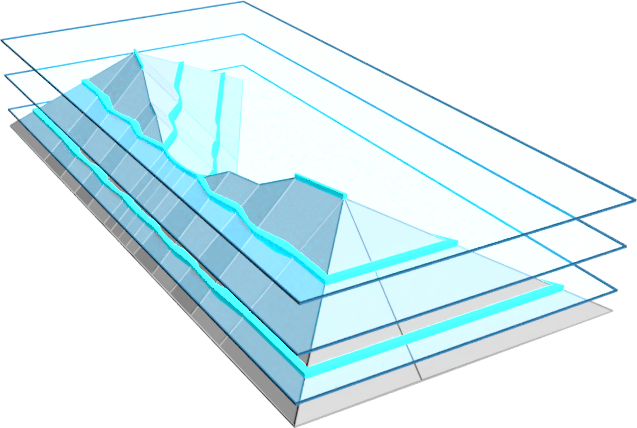
\includegraphics[height=\figheight]{sources/method/overview/surface/sliced_cropped.png}

\vspace{\tempheight}


\includegraphics[width=\figheight]{sources/method/overview/2D/sliced.png}
\caption{Adaptive width paths}\label{3d_surface_overview_sliced}
\end{subfigure}
\caption{
The first row illustrates the generation of uniform paths \subref{overview_uniform_paths}
by interpreting the path as the intersection between horizontal planes and the union of cones \subref{overview_uoc}, which is an alternative visualization of the skeleton \subref{overview_skeleton}. 
The second row depicts the stages with both 2D and 3D visualizations for generating paths with adaptive width \subref{3d_surface_overview_sliced}.
Central elements in the skeleton are first identified (blue in \subref{3d_surface_overview_center}).
The heights are then quantized in terms of number of beads (the integer values in \subref{3d_surface_overview_rounded}), and smoothed \subref{3d_surface_overview_smoothed}.
}
\label{3d_surface_overview}
\end{figure*}

For ease of reference we have included a legend showing the terms employed in this manuscript in \cref{legend}.
These terms will be further explained as they first appear later in this paper. 

\begin{figure}\centering
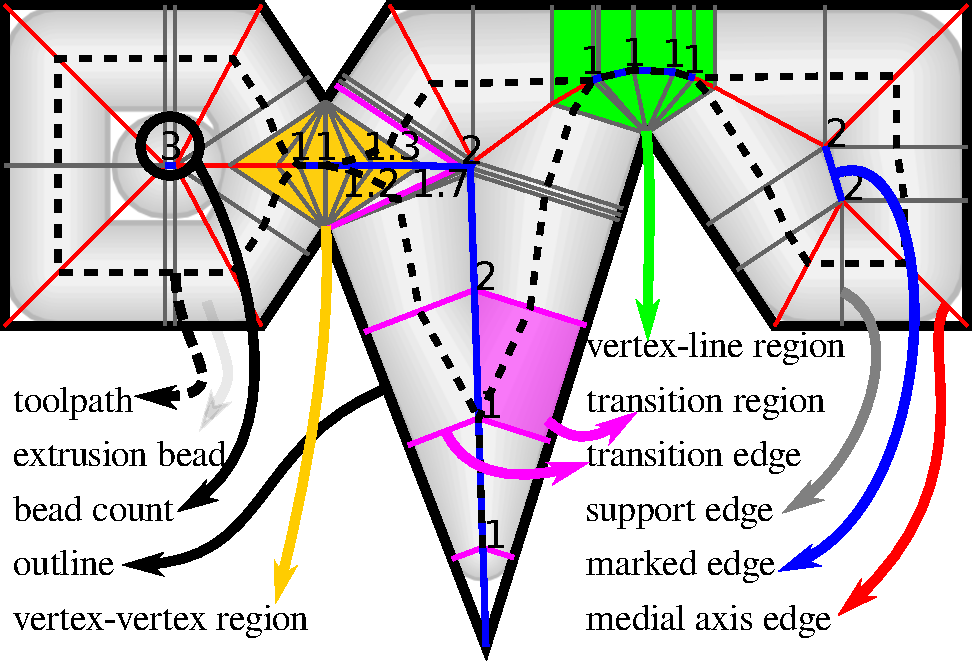
\includegraphics[width=.75\columnwidth]{sources/method/legend2.pdf}
\caption{Illustrative explanation of terms and color coding that are consistently used in this paper.}
\label{legend}
\end{figure}




















%\subsection{Surface generation}\label{sec_surface_construction}
\subsection{Union of cones}\label{sec_surface_construction}

The union of cones (UoC) is derived from a common skeletonization of the polygonal outline shape: the medial axis.
By assigning each node in the skeleton a height equal to its shortest distance to the outline we obtain the shape of the UoC.
Starting from the medial axis we further decompose the shape into simple fragments, so that the domain contains only quads and triangles.
This decomposition constitutes an approximation of the UoC. 


%\subsubsection{Medial axis transform}
\paragraph{Medial axis transform}
The medial axis is a compact and complete representation of a shape.
It is defined as the set of positions where the inscribed circle meets the boundary in at least two locations~\cite{blum1967transformation,lee1982medial}.
The resulting skeleton consists of straight edges and parabolic edges.
An example is illustrated in \cref{shape_decomposition_mat}.
We call the set of points on the outline polygon $P$ closest to a skeletal point $v$ its \emph{support}:
\begin{equation}
    \text{sup}(v) = \argmin_{x\in P} |x - v|.
\end{equation}
The shortest distance for a point on the skeleton is called its feature radius, $R(v)$.
%See \cref{MAT_explanation_circles}.
%We therefore represent the skeleton in a standard half-edge data-structure.
%See \cref{shape_decomposition_datastructure}.
%Alternatively the medial axis can be defined as the locations where the UoC surface is discontinuous~\cite{blum1967transformation}
%The medial axis can therefore be seen as the space within which contour following toolpaths are generated.
%See \cref{MAT_explanation}.
The medial axis along with the feature radius values along the skeleton form a complete shape descriptor, known as the medial axis transform (MAT).
%Feature radius and node locations will be used below to analyse the shape locally.

By vertically raising the center of an inscribed circle to a height that equals the center's feature radius, a cone is formed. 
The union of all such cones forms a 3D solid volume. 
The medial axis can thus also be interpreted as ribs of the surface of the union of cones~\cite{blum1967transformation}.



\begin{figure}\centering
\setlength{\figwidth}{0.24\columnwidth}
\setlength{\figwidthTwo}{0.3\columnwidth}
\begin{subfigure}[t]{\figwidth}\centering
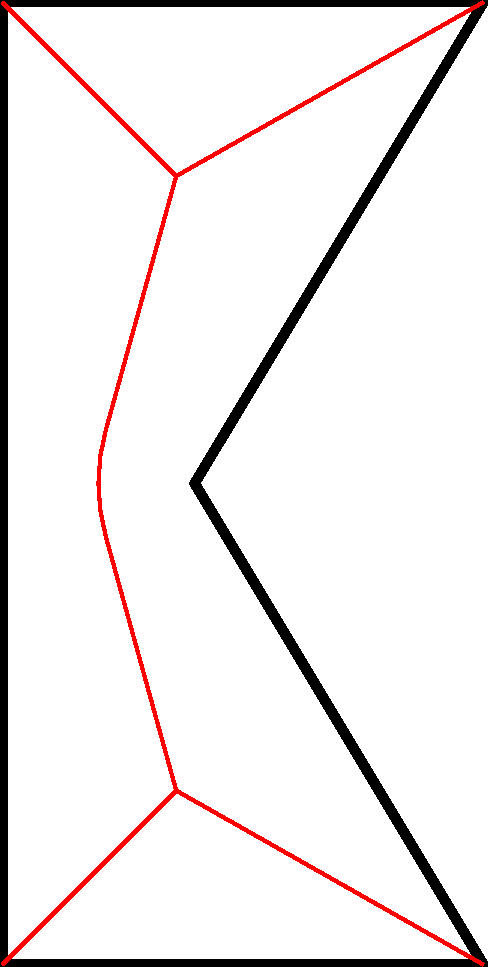
\includegraphics[height=\figwidthTwo]{sources/method/simple_skeleton_mat}
\caption{Medial Axis}\label{shape_decomposition_mat}
\end{subfigure}
\begin{subfigure}[t]{\figwidth}\centering
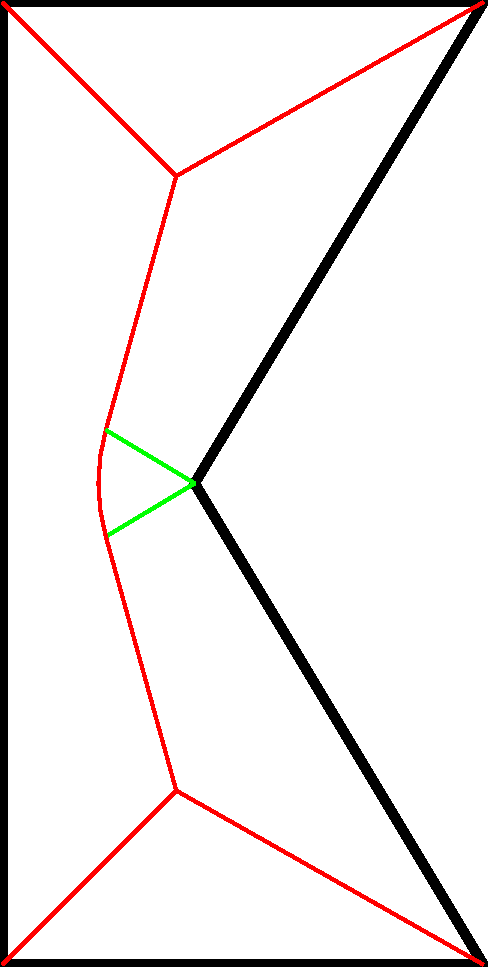
\includegraphics[height=\figwidthTwo]{sources/method/simple_skeleton_vd}
\caption{Voronoi Diagram}\label{shape_decomposition_vd}
\end{subfigure}
\begin{subfigure}[t]{\figwidth}\centering
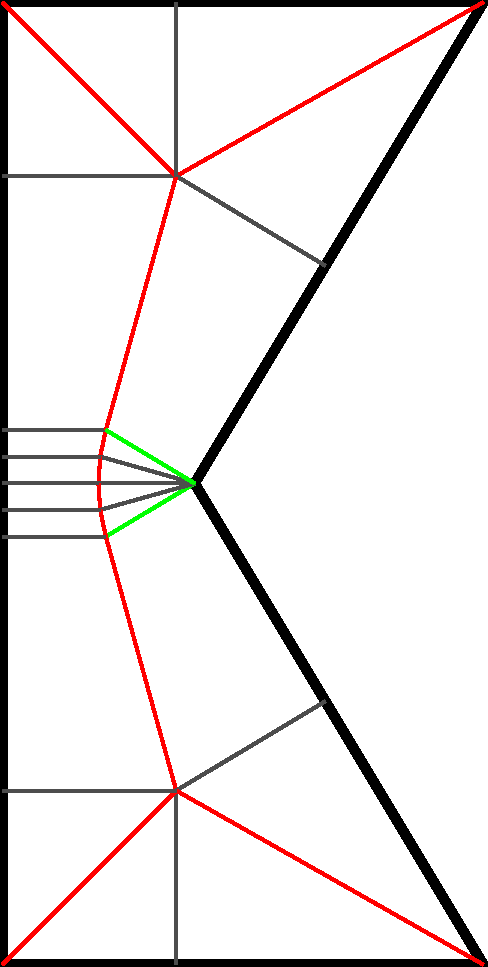
\includegraphics[height=\figwidthTwo]{sources/method/simple_skeleton_st}
\caption{Skeletal Trapezoidation}\label{shape_decomposition_st}
\end{subfigure}
\begin{subfigure}[t]{\figwidth}\centering
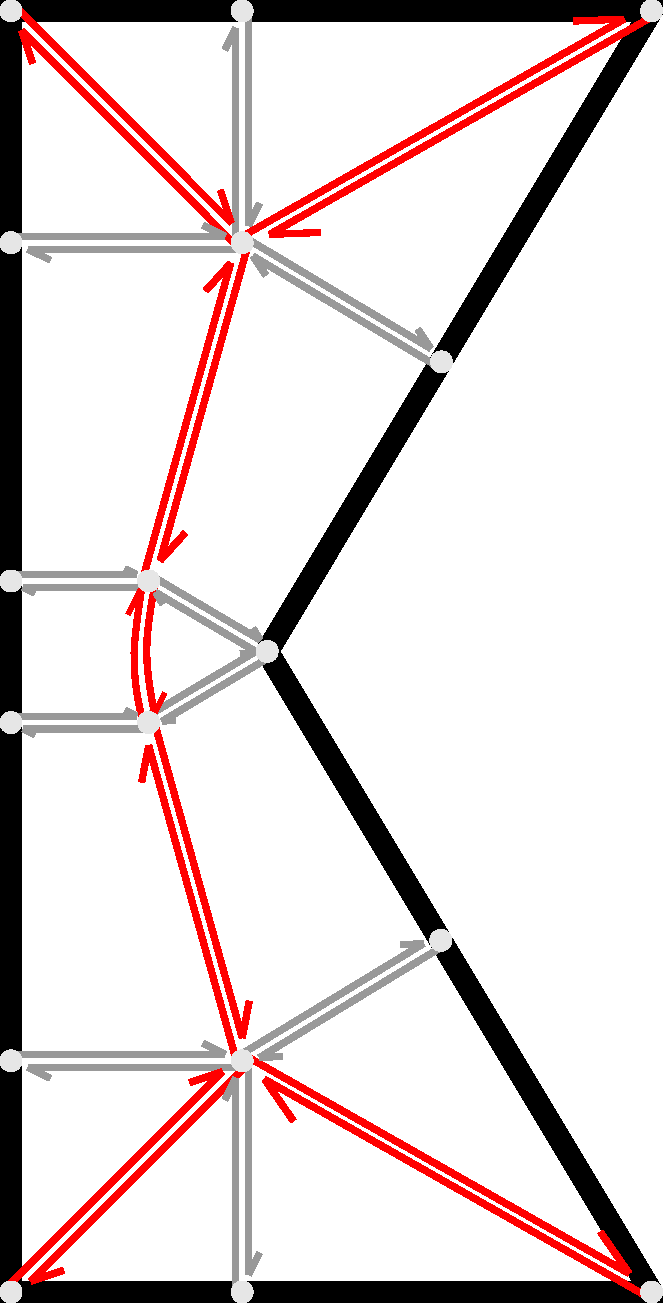
\includegraphics[height=\figwidthTwo]{sources/method/half_edge_datastructure.pdf}
\caption{Data structure}\label{shape_decomposition_datastructure}
\end{subfigure}
\caption{
Skeletonization of an outline shape (black).
Relation between the medial axis (red), the limited Voronoi Diagram (red and green) and the Skeletal Trapezoidation (red, green and gray): MAT $\subset$ Limited VD $\subset$ ST.
\subref{shape_decomposition_datastructure} We can represent a skeleton using a half-edge data-structure.
}
\label{skeletonization_comparison}
\end{figure}



%\subsubsection{Skeletal trapezoidation}
\paragraph{Skeletal trapezoidation}
Starting from the medial axis we decompose the input polygon into a set of quads and triangles, so that we can perform the slicing stage on simple shapes.
We employ a shape decomposition similar to the one proposed by \citeauthor{Ding2016a}~\cite{Ding2016a}. 
The basic idea is to add edges connecting each node $v$ on the medial axis to (all of) its supports, $\text{sup}(v)$. 
The resulting skeleton decomposes the outline shape into trapezoids and triangles.
Considering the fact that the concept of trapezoidation conventionally allows for the degenerate case where a trapezoid resolves into a triangle~\cite{chazelle1984,fournier1984}, we call this shape decomposition the \emph{Skeletal Trapezoidation} (ST).


The edges generated by the MAT can be classified into three types:
\begin{enumerate*}
\item line-line edge -- straight edge generated from two line segments in the outline polygons,
\item vertex-line edge -- parabolic edge resulting from an outline vertex and a line segment in the outline, and 
\item vertex-vertex edge -- straight edge resulting from two outline vertices.
\end{enumerate*}
The vertex-line and vertex-vertex edges are discretized into pieces with a length up to $d^\text{discretization}$.
This allows to approximate the feature radius in between two discretized nodes $v_0$ and $v_1$ by linear interpolation. 
Again we connect the newly inserted nodes to their support, which results in vertex-line regions and vertex-vertex regions such as depicted in \cref{legend}.


% The ST contains all edges from the medial axis which are generated from two line segments in the outline polygons.
% The interaction between an outline vertex and a line segment results in a parabolic edge, which is discretized into pieces with a length up to $d^\text{discretization}$ (see the middle of \cref{shape_decomposition_st}).
% Additionally medial axis edges which are generated from two outline vertices are also discretized, so that the feature radius $R$ in between two discretized nodes $v_0$ and $v_1$ can be approximated by linear interpolation between $R(v_0)$ and $R(v_1)$.
% Again we connect the nodes which are introduced by the discretization to their support, which results in vertex-line regions and vertex-vertex regions such as depicted in \cref{legend}.



%\subsubsection{Union of cones}
\paragraph{Approximation of union of cones}
The skeleton trapezoidation (ST) provides a means to visualize the union of cones (UoC) approximated by a 3D surface mesh composed of quadrilateral and triangular patches.
%In order to visualize the ST as a 3D surface, we add a third dimension.
We assign each node in ST a (real number) height value measured in terms of beads, referred to as the \emph{bead count} $b$.
We define the bead count as the number of beads to fit along the \emph{diameter} of the inscribed circle centered at node $v$, i.e. $2R(v)$, by
\begin{equation}
    \tilde{b}_v = 2 R(v) / w^*
\label{eq:initialBeadCount}
\end{equation}
where $w^*$ is the nozzle size. 
%While the feature radii are measured along the support edges, the diameter is not measurable as such because the support edges are generally not collinear;
We divide the diameter rather than the radius as this allows to deal with an odd number of beads while using integer logic.
%The result is a mesh representing the union of cones (UoC) consisting entirely of quads and triangles.
Note that although the overview of the method has been described geometrically in terms of the UoC, the actual toolpath generation relies on the two-dimensional ST, while the use of the bead count as a height value is only a visualization aid.







\paragraph{Implementation}
The medial axis of a polygonal shape is a subset of the Voronoi Diagram generated from the line segments and vertices of the shape~\cite{lee1982medial}. 
The edges of the Voronoi diagram that fall outside of the outline shape are irrelevant for our purpose and thus discarded.
Note that the Voronoi diagram contains, in addition to the medial axis, edges connecting to concave vertices in the outline shape (see \cref{shape_decomposition_vd}). 
These extra edges are a subset of the edges connecting a node to its support, so we keep them in.
From the Voronoi diagram we add nodes to discretize parabolic edges and edges formed by two concave outline vertices, and then connect all nodes to their supports, forming a skeletal trapezoidation. 
We then assign each node the bead count values using \cref{eq:initialBeadCount}.
We compute the Voronoi diagram using the Boost \verb!C++! libraries~\cite{schaling2011boost}, which implements the algorithm proposed by \citeauthor{fortune1986sascg}~\cite{fortune1986sascg}.
A half-edge data-structure is used to represent the Voronoi diagram (\cref{shape_decomposition_datastructure}).

%









\subsection{Center classification}\label{sec_center_classification}
%The simple technique of performing uniform width offset produces large overfill and underfill areas on central regions of the ST.
%These central regions present themselves as upper ridges in the mountains of the UoC surface.
%In order to prevent the over- and underfill we will change the bead counts in the central regions.
%This sections covers what parts of the UoC will be marked as being central.
In order to prevent over- and underfill to occur in central, we mark parts of the ST as being central.
The remainder is called peripheral.
Our framework will decide on a beading at all of the marked nodes in `the center' and apply the beading outward to the unmarked nodes (\cref{sec_peripheral_height_adjustment}).

We mark a node in the ST as central if its feature radius is larger than that of all its neighboring nodes, i.e. a local maxima.
%That is: we mark the local maxima, i.e. the mountain tops of the UoC as being central.
We also mark an edge as being central if it is significant according to a significance measure.

%\subsubsection{Significance measure}\label{sec:significance_measure}
\paragraph{Significance measure}
We make use of the \emph{bisector angle} as an indicator of significance which is commonly used in shape analysis.
%Centrality can be formalized by looking at a commonly used significance measure knows as the \emph{bisector angle}.
The bisector angle $\alpha$ is the interior angle $\angle{p_0lp_1} \leq \SI{180}{\degree}$, between any location $l$ on an edge of the ST and its two supporting points $ \{ p_0, p_1 \} = \text{sup}(l)$~\cite{attali1996modeling}. 
An edge is significant if the bisector angle on any location on the edge exceeds a prescribed $\alpha_\text{max}$. 
As illustrated in See \cref{naive_overfill_underfill}, for a polygon with a pointy wedge area of an angle $\beta$, we have $\alpha = 180\degree - \beta$. This corresponds to overfill areas and underfill areas the size of $\nicefrac12 (w^*)^2 \left( \nicefrac14 \tan ( \alpha / 2) - \alpha / 2 \right)$ when filled using the simple technique of uniform bead width $w^*$.
Although significance measures are commonly used as a heuristic for finding the parts of a skeleton which are in some sense relevant~\cite{attali1996modeling,Sud2007},
we use the bisector angle as an \emph{exact} indicator of the amount of overfill and underfill in the uniform toolpaths of constant width.
%Contrary to related literature we will \emph{keep} the non-significant regions of the skeleton.
%We mark all significant edges as such and contrary to related literature we keep the unmarked edges of the ST.


\begin{figure}
\centering
\setlength{\figheight}{.3\columnwidth}
\begin{subfigure}{0.45\columnwidth} \centering
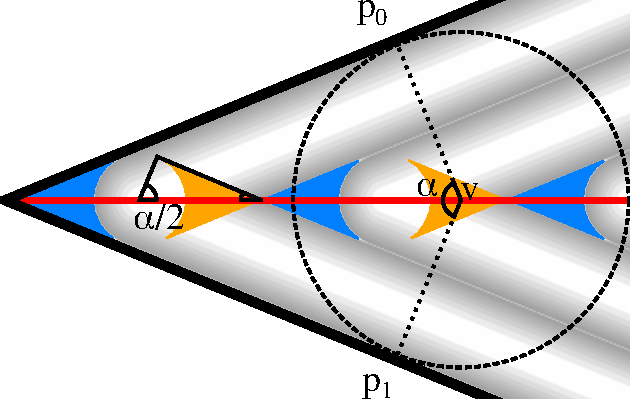
\includegraphics[height=\figheight,frame]{sources/method/naive_overfill_underfill.pdf}
\caption{Over- and underfill}\label{naive_overfill_underfill}
\end{subfigure}
\begin{subfigure}{0.45\columnwidth} \centering
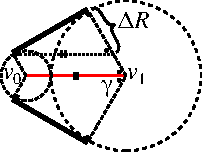
\includegraphics[height=.8\figheight]{sources/method/significance_properties.pdf}
\caption{Significance measure}\label{distance_based_angles}
\end{subfigure}
\caption{
Properties of the significance measure along a skeletal edge (red) generated from two polygon lines (black) using the properties of inscribed circles (gray) and their radii (dashed).
\subref{naive_overfill_underfill}
The size of overfill (orange) and underfill areas (azure) for the uniform toolpathing technique can be calculated from the bisector angle.
% $a = 180\degree - \beta$ is the angle between a location $v$ and its support $p_0$ and $p_1$.
\subref{distance_based_angles}
The significance measure can be simplified using $\alpha = 2 \gamma = 2 \cos^{-1} \Delta R / |v_1 - v_0|$.
}
\end{figure}

% The significance evaluation is performed efficiently by checking the ratio between feature radius $R$ and the Euclidean distance:
% if $ | R(v_1) - R(v_0) | / |v_1 - v_0| >  \cos(\alpha_\text{max} / 2)$ then $\alpha > \alpha_\text{max}$. See \cref{distance_based_angles}. This ratio has a clear geometrical interpretation as the slope of the ridge in the UoC surface.

To avoid evaluating the bisector angle at any location on all edges, we devise an efficient measure which operates only on the two nodes of an edge.
Because all locations along a line-line edge have the same bisector angle we can evaluate whether the edge is significant by checking whether 
\begin{align}\label{simple_significance_measure}
| R(v_1) - R(v_0) | / |v_1 - v_0| >  \cos(\alpha_\text{max} / 2)
\end{align}
(see \cref{distance_based_angles}).
This ratio has a clear geometrical interpretation as the slope of the ridge in the UoC surface.
For vertex-line edges and vertex-vertex edges only a portion of the edge may be significant.
We therefore introduce nodes at the boundaries of the significant portion during the discretization of such edges (see Appendix~\ref{edge_discretization}).
The significance of all edges can then accurately be evaluated using \cref{simple_significance_measure}.






%\subsubsection{Marking filtering}
\paragraph{Marking filtering}
After initializing the marking at all edges and nodes, we filter out high frequency changes in the marking in order to ensure that the generated toolpath is smooth. 
The filtering is performed by additionally marking some unmarked elements, rather than the opposite since unmarking central regions reintroduce large over- and underfill areas.
From each marked node $v_0$ with an upward unmarked edge attached we walk along the upward edges;
if the total length traversed until we reach another marked node $v_1$ is shorter than some filter distance $d_\text{max}^\text{unmarked}$, we mark all edges encountered as being central.















\subsection{Central height adjustment}\label{sec_central_height_adjustment}
Now that we have identified and marked the central regions we quantize their heights.
We first quantize the initial bead count $\tilde{b}$ into an integer bead count $\bar{b}$ at the marked nodes using a quantization operator $q$,
then find the locations along the edges where $q$ makes a jump from one bead count $n$ to another $n+1$
and then introduce ramps to smoothly transition from $n$ to $n+1$ using fractional bead counts $\hat{b}$ along the smooth transition.
%\subsubsection{Initial bead count}\label{sec_initial_bead_count}



\begin{figure*}
\centering
\setlength{\figwidth}{0.13\textwidth}
\begin{subfigure}{\figwidth}
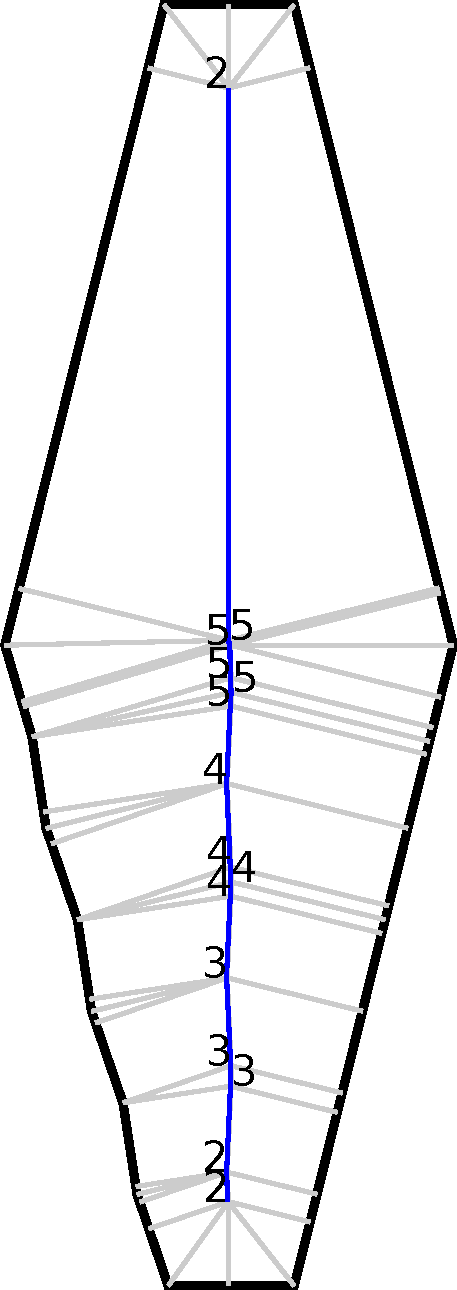
\includegraphics[width=\columnwidth]{sources/method/beading_transitioning_filtering__bead_count.pdf}
\caption{Quantized bead counts}\label{beading_transitioning_filtering__bead_count}
\end{subfigure}
\begin{subfigure}{\figwidth}
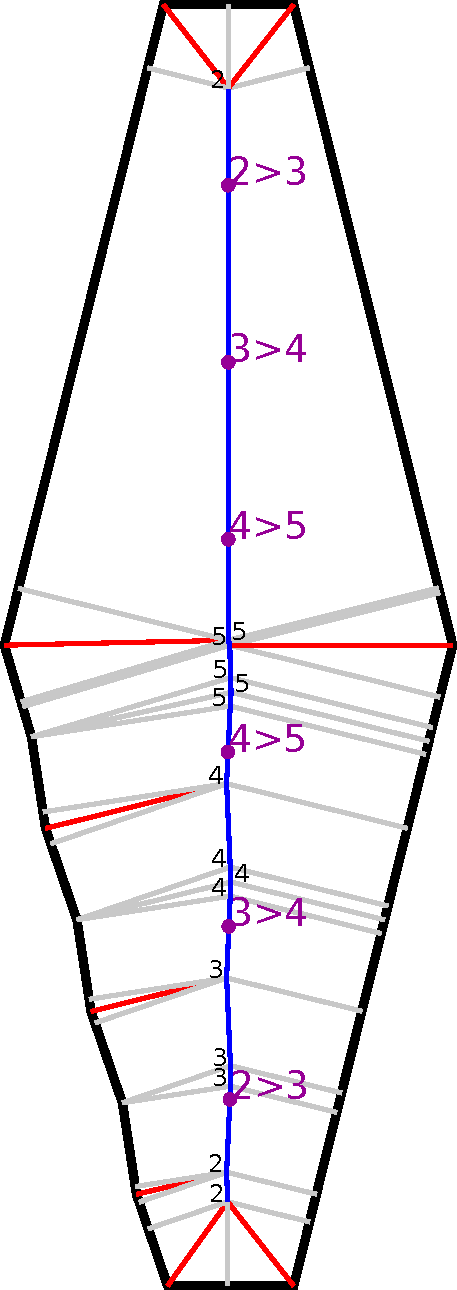
\includegraphics[width=\columnwidth]{sources/method/beading_transitioning_filtering__transition_mids.pdf}
\caption{Transition anchors}\label{beading_transitioning_filtering__transition_mids}
\end{subfigure}
\begin{subfigure}{\figwidth}
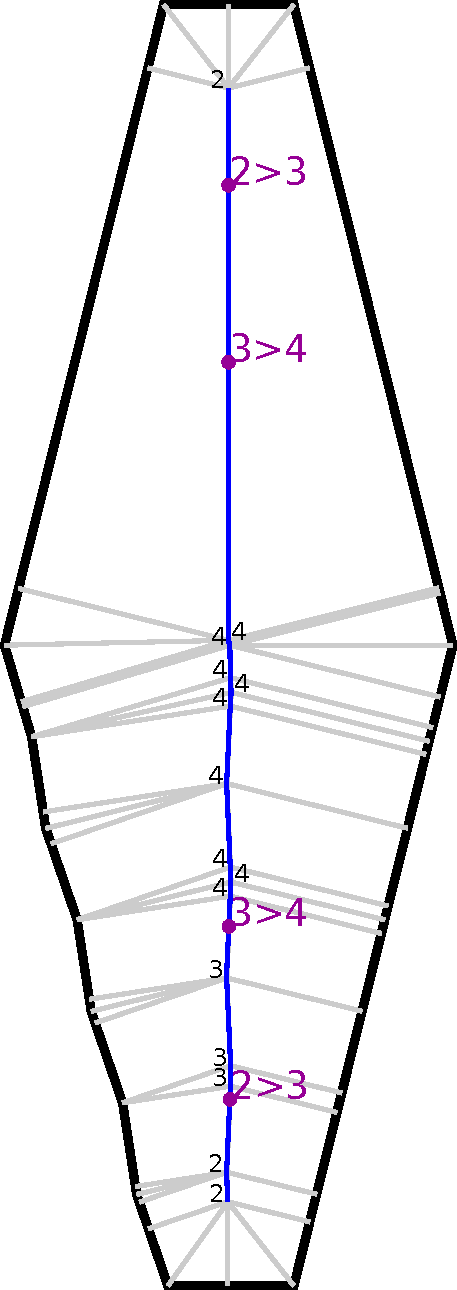
\includegraphics[width=\columnwidth]{sources/method/beading_transitioning_filtering__filtered.pdf}
\caption{Filtered anchors}\label{beading_transitioning_filtering__filtered}
\end{subfigure}
\begin{subfigure}{\figwidth}
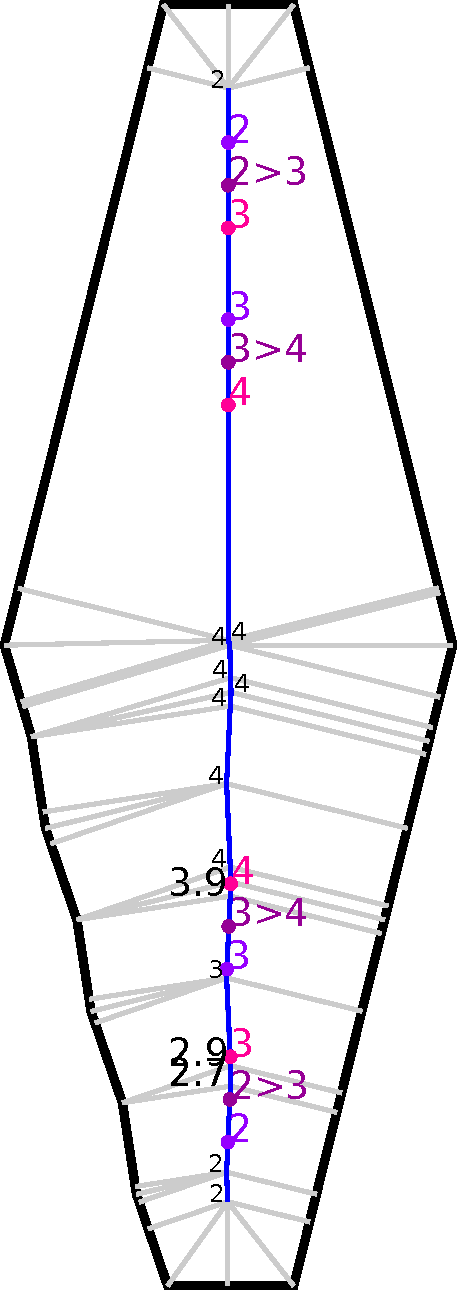
\includegraphics[width=\columnwidth]{sources/method/beading_transitioning_filtering__transition_ends.pdf}
\caption{Transition ramp ends}\label{beading_transitioning_filtering__transition_ends}
\end{subfigure}
\begin{subfigure}{\figwidth}
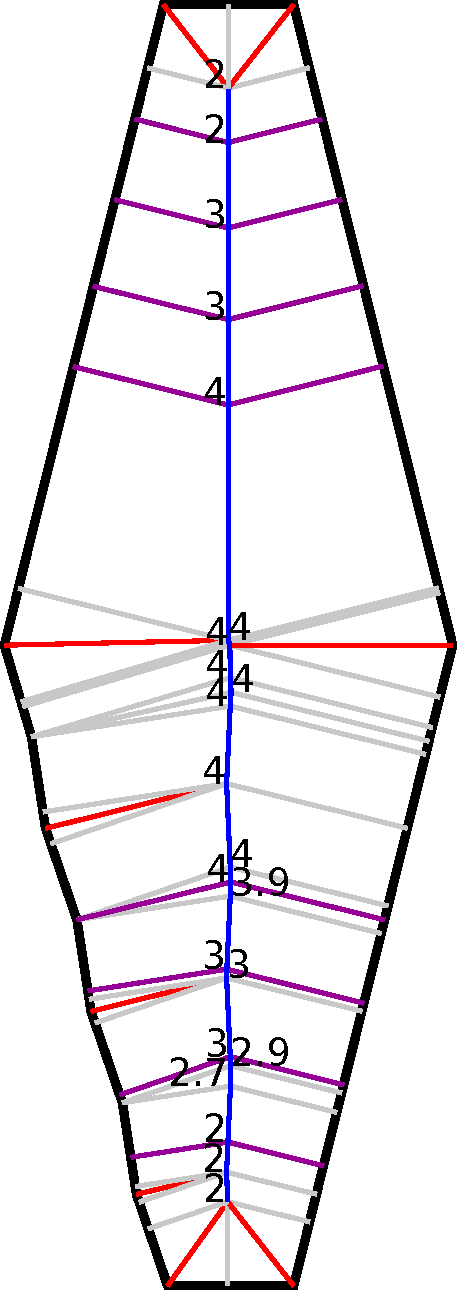
\includegraphics[width=\columnwidth]{sources/method/beading_transitioning_filtering__transitions_applied.pdf}
\caption{Radial support edges}\label{beading_transitioning_filtering__transitions_applied}
\end{subfigure}
\begin{subfigure}{.27\textwidth}
\hspace*{-.5cm}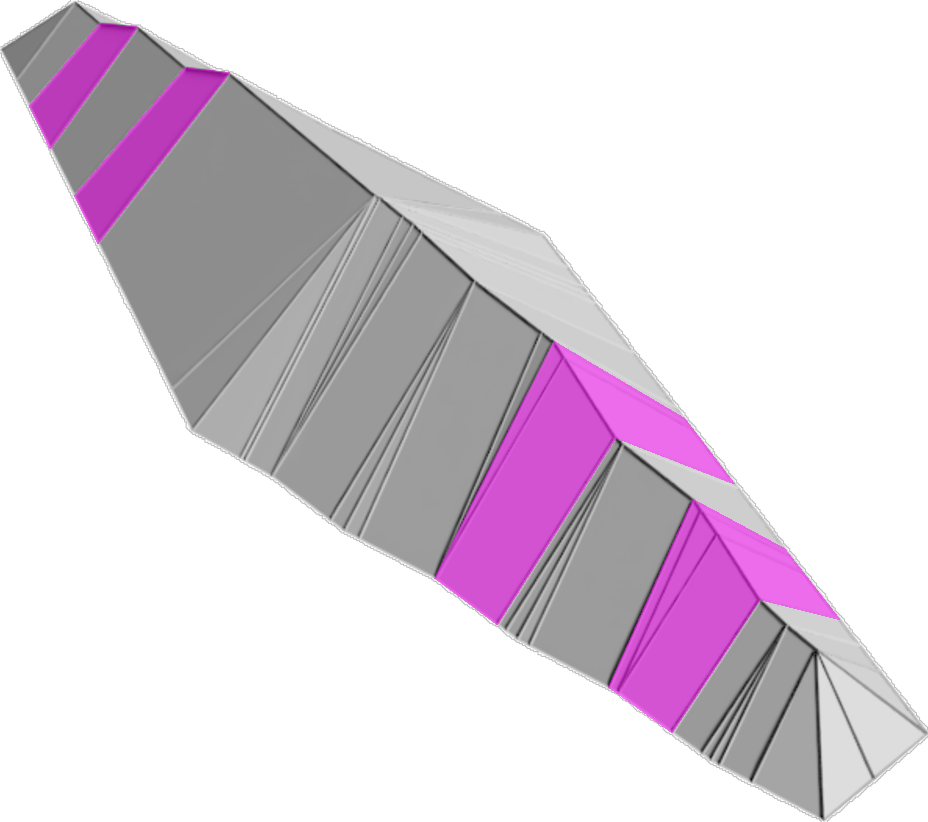
\includegraphics[width=1.2\columnwidth]{sources/method/beading_transitioning_filtering__result_uoc.pdf}
\caption{Result UoC}\label{beading_transitioning_filtering__result_uoc}
\end{subfigure}
\caption{
Applying bead counts and transitioning on a shape showing the difference between a simple ST (top) and a mirrored version with small perturbations in the outline (bottom).
Outline in black, medial axis edges in red, radial edges in grey.
\subref{beading_transitioning_filtering__bead_count} First we initialize the bead counts (black) in the marked regions (blue).
\subref{beading_transitioning_filtering__transition_mids} We then extract the anchor locations (purple) of the transitions to a different bead count should be.
\subref{beading_transitioning_filtering__filtered} We then filter out regions of constant bead count.
\subref{beading_transitioning_filtering__transition_ends} We then calculate the end locations (magenta, pink) of the transitions and modify the bead count at nodes in between to fractional values.
\subref{beading_transitioning_filtering__transitions_applied} Finally we introduce nodes at the ends and introduce radial edges (purple) as per the trapezoidation constraint.
The symmetry in the result shows that transitioning is robust against small perturbations in the outline shape.
}
\label{beading_transitioning_filtering}
\end{figure*}


%\subsubsection{Quantization}

\paragraph{Quantization}
We define a quantization operator $q$ to map a feature diameter ($d=2R(v)$) to a bead count: $q: \mathbb{R} \to \mathbb{N}$.
Because our quantization scheme should round to the nearest integer multiple of the nozzle size, we have
$q(d) = \left\lfloor d / w^* + \nicefrac12 \right\rfloor$.
Alternative quantization schemes will be discussed in \cref{sec_generalization}.
By applying $q$ to the heights of central nodes we quantize the bead count:
\begin{equation}\label{eq_quantized_bead_count}
\bar{b}_v = q(2R(v)) = \left\lfloor \tilde{b}_v + \nicefrac12 \right\rfloor
\end{equation}

\iffalse
Along with this quantization, an amendment to the marking filtering is performed, in order to alleviate a problem that will be handled in \cref{section_beading_conflicts}.
Specifically, unmarked regions are marked as central if they lie between two nodes with the same integer bead count.
\fi
%We then filter out short unmarked regions where the bead count remains constant in order to limit the extent of a problem handled in \cref{section_beading_conflicts}.
% From each marked node $v_0$ with an upward unmarked edge attached we walk along the upward edges until we hit another marked node $v_1$.
% If the upper node has the same bead count $b^*_{v_1} = b^*_{v_0}$ we mark all edges and nodes $v$ in between, and set the bead count $b^*_v \leftarrow b^*_{v_0}$.

\paragraph{Transition anchors}
For a marked edge which connects nodes $v_0$ and $v_1$ with $\bar{b}_{v_0} \le n < \bar{b}_{v_1}$, we determine the \emph{transition anchor locations} at which the bead count transitions from $n$ to $n+1$.
To this end, we introduce the function 
\begin{equation}
    q^{-1}(n) := \argmax_d q(d) = n,
\end{equation}
which gives the feature diameter $d$ at which the bead count $q$ transitions from $n$ to $n+1$.
The location of the anchor $v_x$ is then computed by inversely interpolating $R(v_x) = q^{-1}(n)$, i.e. 
\begin{equation}
    v_x = v_0 + (v_1 - v_0) \frac{ q^{-1}(n) - R(v_0) }{ R(v_1) - R(v_0) }.
\end{equation}
%for each $n$ such that $b^*_{v_0}\le n<b^*_{v_1}$.
An illustration of the anchors is shown in \cref{beading_transitioning_filtering__transition_mids}.

We perform a filtering step to prevent frequently changing the bead count back and forth within a short distance.
For two consecutive anchors which transition to opposite directions, if the distance between them is smaller than some limit $d_\text{max}^\text{transition}$, the bead counts at all nodes in-between are set to the surrounding bead counts, and consequently these anchors are removed (See \cref{beading_transitioning_filtering__filtered}).

% For each edge which contains a transition anchor we walk along the marked edges until we encounter another anchor.
% If the other anchor is a transition in the opposite direction and the traversed distance is within some limit $d_\text{max}^\text{transition}$ we remove the transitions and set the bead counts at all nodes in the filtered region to the surrounding bead counts.
% See \cref{beading_transitioning_filtering__filtered}.






% \subsubsection{Smooth transition}
\paragraph{Smooth transitions}

A sharp transition from $n$ to $n+1$ beads at an anchor location creates sharp turns in the toolpath (see \cref{transitions} top).
A transition length $t(n)$ is introduced to ensure a smooth transition (see \cref{transitions}). 
The length of the transition is set to $t(n) = w^*$ and it is centered at the anchor, i.e. the distance from the lower end $v_0$ to the anchor position $v_x$ is set to
$t_0(n) = \Delta(v_0v_x) = \nicefrac12 w^*$,
where $\Delta$ is the total distance along the edges in between two nodes.
We discard any transition anchor which is too close to the end of a chain of marked edges for the smoothed transition to fully fit within the marked region.
In order to make the transition ramps robust against small perturbations in the outline shape which cause extra (support) edges in the skeleton,
we modify the nodes $v_x$ which are in between the two ends $v_0$ and $v_1$ of the transition by (re-)assigning them a fractional bead count $\hat{b}$ which is linearly interpolated between the two ends of the transition (see \cref{beading_transitioning_filtering__transitions_applied}):
\begin{equation}
\hat{b}_{v_x} = n + {\Delta(v_0v_x)} / {\Delta(v_0v_1)}
\end{equation}
Note that although the ST is not stable against noise in the boundary shape, the distance field itself is, so by designing our algorithms such that they are stable against changes in the topology of the skeleton our method is stable against small perturbations in the outline.
%This modification makes the transition ramps robust against small perturbations in the outline shape (to be explained in \cref{section_beading_interpolation});
%compare the top and bottom of \cref{beading_transitioning_filtering}. 
Finally we update the ST by adding support edges at the transition ends. 
As shown in \cref{beading_transitioning_filtering__result_uoc}, the marked regions in the UoC mesh have become horizontal at integer multiples of $\nicefrac12 w^*$ for long stretches with ramps in between.




\begin{figure}
\centering
\setlength{\figwidth}{\columnwidth}
\begin{subfigure}{0.9\figwidth}\centering

\includegraphics[width=\columnwidth]{sources/method/wedge_no_transitioning.png}
\caption{Without transitioning}
\end{subfigure}
\begin{subfigure}{0.9\figwidth}\centering

\includegraphics[width=\columnwidth]{sources/method/wedge_transitioning.png}
\caption{Transitioning}
\end{subfigure}
\caption{
Discontinuities around regions where the bead count changes are prevented by transition regions (highlighted in cyan).
}
\label{transitions}
\end{figure}














\subsection{Beading}\label{sec_peripheral_height_adjustment}
Now that we have determined the bead counts in the central regions we will describe how the peripheral regions are handled.
Determining bead count values for the unmarked nodes and interpolating linearly along the unmarked edges would mean that toolpath sites would be distributed evenly along each unmarked bone;
while that would suffice for the evenly distributed beading scheme, it wouldn't allow for more sophisticated, non-linear schemes (see \cref{peripheral_heights}).
Instead we determine the radial distance to the boundary at which each bead should occur.
Each central node is associated with a sequence of radial distances $L$ which control the locations of the beads, startign from the outer bead and ending in the center.
Together with a sequence of bead widths $W$ these form what we call a \emph{beading} $B$.
For our distributed beading scheme we compute the beading for a central node $v$ with $n = \hat{b}_v$ beads and a diameter $d = 2R(v)$  as:
\begin{align*}
    B(n,d) &= \left( W(n,d), L(n,d) \right)   &=   \left( \left\{  w_0 , \dots, w_{n-1} \right\}, \left\{ l_0 , \dots, l_{n-1} \right\} \right) \\
    w_i &= 2R(v) / n  & \text{for all $i < n$}\\
    l_i &= 2R(v) / n (i + \nicefrac12) & \text{for all $i < n$}
\end{align*}
where
$w_i$ and $l_i$ are the width and location of the $i$th bead,
respectively, counting from the outline inward.
An example beading is visualized in the top of \cref{beading_interpolation}:
$B^V$ cover the total horizontal distance $d$ using $n=4$ beads all with the same width and radial locations $l$ evenly divided over the length $d$.




\begin{figure}\centering
\setlength{\figheight}{.2\columnwidth}
\begin{subfigure}{.55\columnwidth}\centering
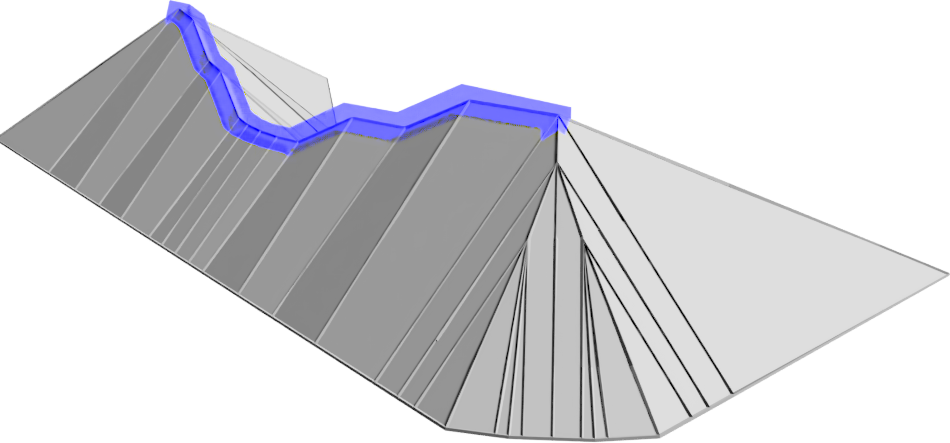
\includegraphics[height=\figheight]{sources/method/peripheral_heights_3D.png}
\caption{Surface mesh}
\end{subfigure}
\begin{subfigure}{.4\columnwidth}\centering
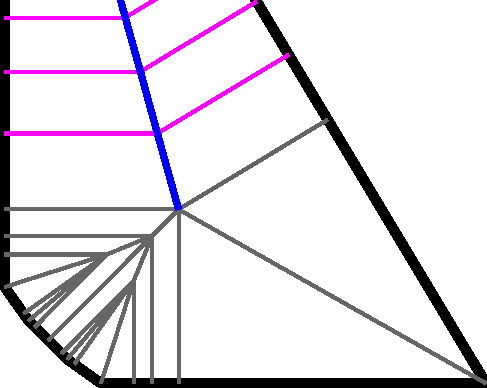
\includegraphics[height=\figheight]{sources/method/peripheral_heights.pdf}
\caption{ST}
\end{subfigure}
\caption{
Shallow corners will cause peripheral nodes for which the height should be determined based on the central node above it.
}
\label{peripheral_heights}
\end{figure}


\paragraph{Beading interpolation}
The beading is defined in terms of an integer number of beads, while we have assigned a fractional bead count to nodes within a transition region.
In order to generate a beading for a node $v$ with $n < b^*_v < n+1 $ we linearly interpolate the bead width and location of the first and last $n/2$ lines between a beading $B^V$ based on $n$ and a beading $B^W$ based on $n+1$ (see \cref{beading_interpolation}).
Such interpolation is also used to deal with beading conflicts (see \cref{beading_conflict_problem}).
We therefore also apply beading interpolation from a marked node $v_m$ upward along unmarked bones,
and interpolate between $v_m$ and the beading at the top of the slope over some distance $t_\text{beading}$ from the lower marked node.

\paragraph{Beading propagation}
The beading information is then broadcasted throughout the ST from central regions outward,
so that each unmarked node $v$ knows the beading of the marked node on top of the ramp on which $v$ is placed.
We first broadcast the beading information upward from all marked nodes,
so that we can then deal with beading conflicts in a downward phase.
This the downward phase makes sure that all nodes have a beading associated with it, so that the slicing algorithm can efficiently slice the edges leading up to a marked or unmarked node.	



\begin{figure}
\centering
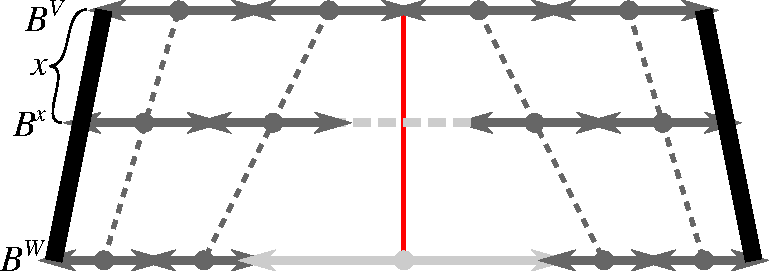
\includegraphics[width=.8\columnwidth]{sources/method/beading_interpolation_v2.pdf}
\caption{
Interpolation between two beadings $B^V$ and $B^W$ with a ratio $x$ results in a beading $B^x$.
Distances between the thick black lines constitute diameters $d$,
the toolpath locations are visualized as dots,
the widths are visualized as bidirectional arrows
and the middle is highlighted in red.
}
\label{beading_interpolation}
\end{figure}

\begin{figure}\centering
\setlength{\figheight}{.2\columnwidth}
\begin{subfigure}{.45\columnwidth}\centering
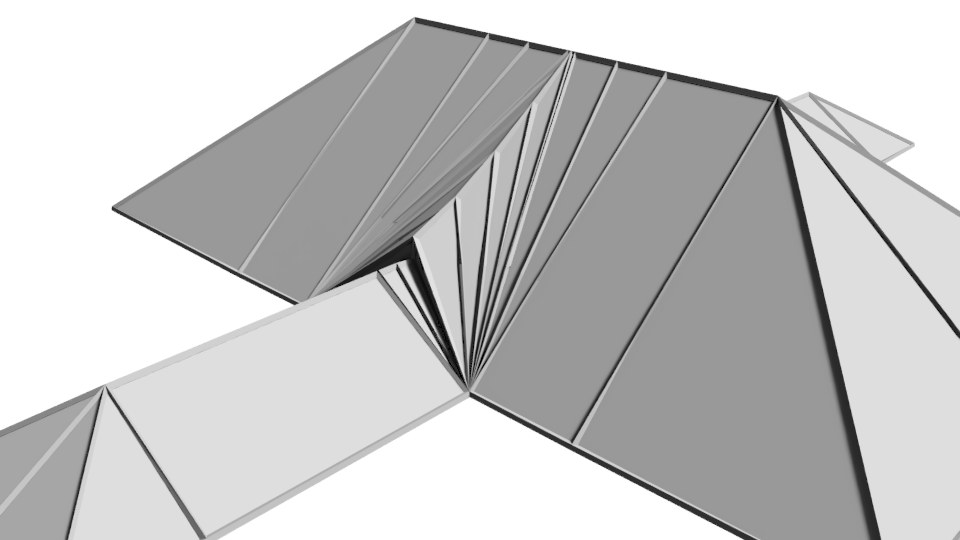
\includegraphics[width=.95\columnwidth,frame]{sources/method/beading_conflict_3D.png}
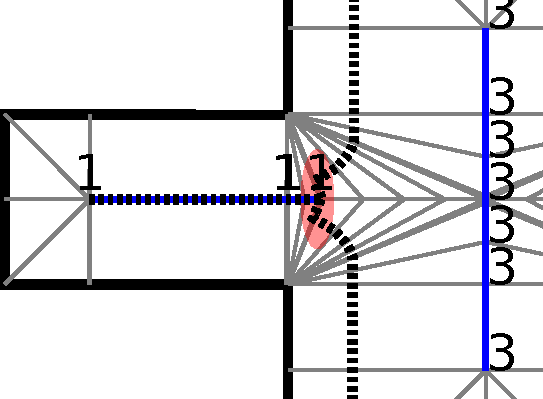
\includegraphics[height=\figheight]{sources/method/beading_conflict.pdf}
\caption{Beading conflict}\label{beading_conflict}
\end{subfigure}
\begin{subfigure}{.45\columnwidth}\centering
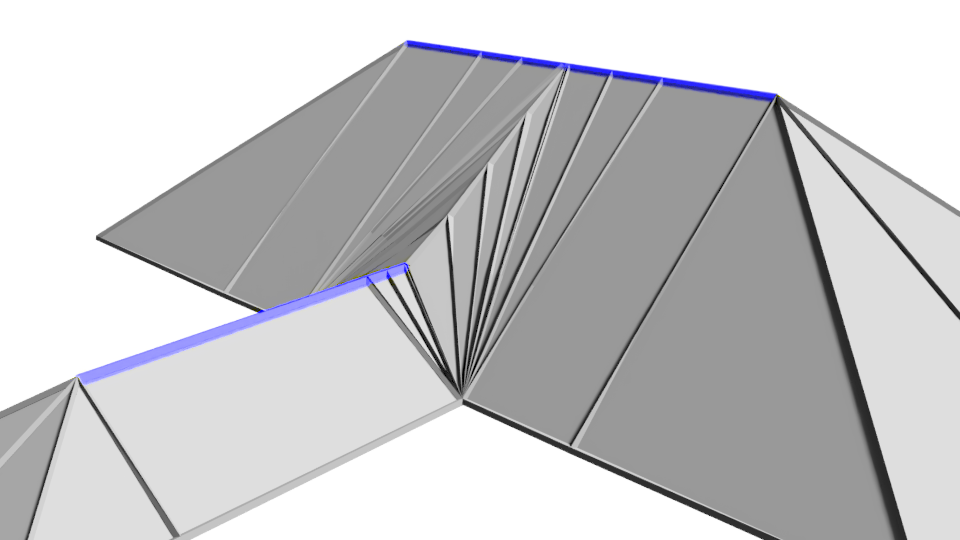
\includegraphics[width=.95\columnwidth,frame]{sources/method/beading_conflict_solved_3D.png}
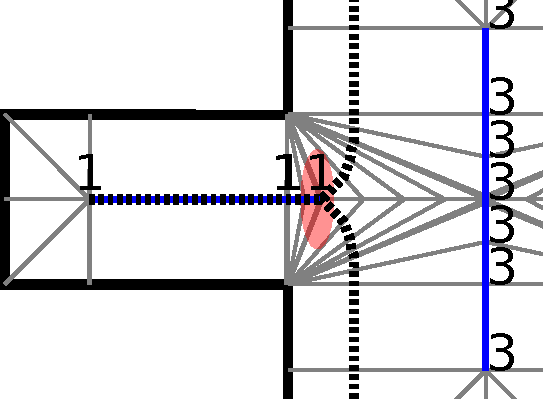
\includegraphics[height=\figheight]{sources/method/beading_conflict_solved.pdf}
\caption{Conflict resolution}\label{beading_conflict_solved}
\end{subfigure}
\caption{
\subref{beading_conflict} The beading propagated from above conflicts with the beading below.
\subref{beading_conflict_solved} The beading conflict is resolved by gradually interpolating between the two beadings.
The ramp to the upper ridge doesn't line up with the lower ridge, which means that
the toolpaths (dashed) resulting from the beading propagated from above doesn't align with the beading from the thin outline feature (highlighted in red).
}
\label{beading_conflict_problem}
\end{figure}








\subsection{Toolpath extraction}\label{sec_toolpath_extraction}
Now that each node has been assigned a beading we proceed to generate the toolpath sites along the edges of the ST.
A site $S$ consists of a location $v$ a width $w$ and an index $i$, which are computed for an edge $v_0v_1$ from the beading $B$ of the upper node $v_1$:
\begin{align*}
S &= \{ v, w, i \} \\ 
v &= v_1 + (v_0 - v_1) \frac{R(v_1) - l_i^B}{R(v_1) - R(v_0)} \\ 
w &= w_i^B
% \\ i^S &= i
\end{align*}
for any $i$ for which $R(v_0) < l_i^B \leq R(v_1)$.
See \cref{site_placement}.
We store all sites of an edge in a mapping from edge to a list of sites.


\begin{figure}
\centering
\setlength{\figheight}{.29\columnwidth}
\begin{subfigure}{0.14\columnwidth}\centering
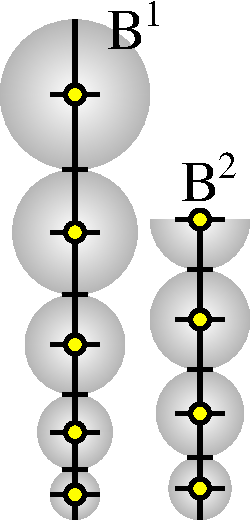
\includegraphics[height=\figheight]{sources/method/trapezoid_beading_beading.pdf}
\caption{Beadings}\label{trapezoid_beading_beading}
\end{subfigure}
\begin{subfigure}{0.5\columnwidth}\centering
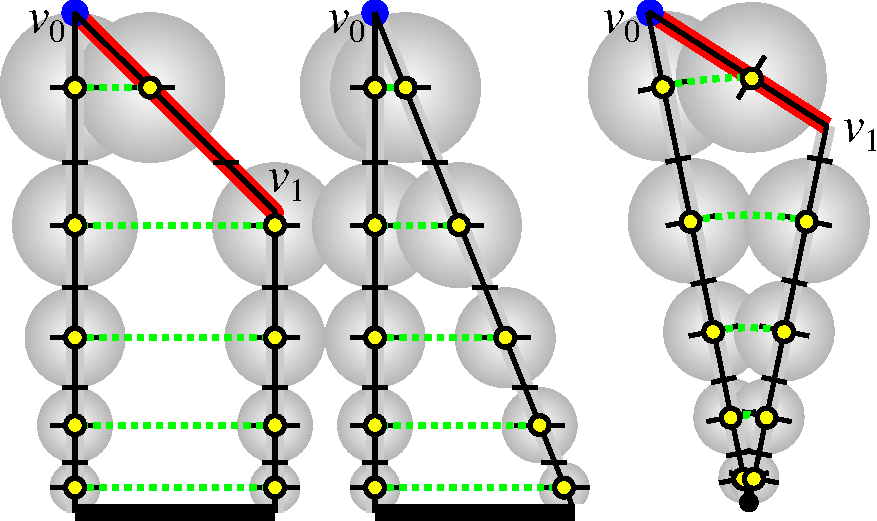
\includegraphics[height=\figheight]{sources/method/trapezoid_beading_propagated.pdf}
\caption{Single beading propagated to all nodes}\label{trapezoid_beading_propagated}
\end{subfigure}
\begin{subfigure}{0.34\columnwidth}\centering
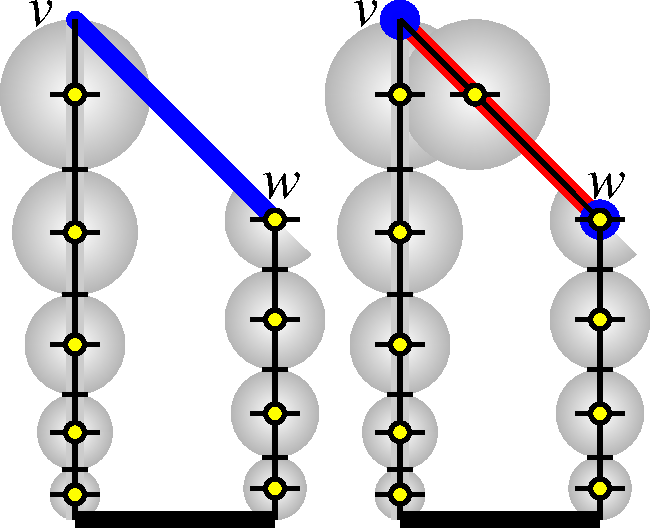
\includegraphics[height=\figheight]{sources/method/trapezoid_beading_separate.pdf}
\caption{Separate beadings at either top node}\label{trapezoid_beading_separate}
\end{subfigure}
\caption{
Applying beadings to generate sites along trapezoids.
\subref{trapezoid_beading_beading} shows half of the locations $l_i$ and widths $w_i$ of two arbitrary different beadings.
\subref{trapezoid_beading_propagated} shows the application of $B^1$ to the various types of trapezoid.
\subref{trapezoid_beading_separate} shows how a trapezoid with a marked edge will have two different beadings assigned, which will generate their respective sites along the support edges.
No sites will be generated along marked edges.
Wide black lines are outline segments, marked nodes and edges in blue, the sites in yellow and green wavefronts of equidistant radial distance at $R = l_i$.
}
\label{site_placement}
\end{figure}


We then generate extrusion segments for each trapezoid by connecting together the sites of the same index.
See \cref{segment_generation}.
If the amount of sites on both sides of the trapezoid is not the same then this trapezoid is in a transition and we leave one inner site unconnected.

Because the bead count is defined in terms of the feature diameter rather than the radius, only some of the bead count values $\hat{b}$ in a central region coincide with a slicing height.
When the bead count $\hat{b}$ is even, the ridge will be sliced as normal;
the intersection between a slicing plane and the mesh surface results in a polyline on both sides of the ridge, which are connected together into a polygonal toolpath.
When the bead count $\hat{b}$ is odd, the ridge will coincide exactly with a slicing height, which results in a single polyline toolpath being generated along the middle of the feature.
In that case we should prevent the algorithm from generating the center extrusion segment twice from the trapezoids on either side of that segment.
We therefore use some arbitrary condition to decide which one of the two to include based on the ordering of the coordinates of $v_0$ and $v_1$: $x_0 < x_1 \lor (x_0 = x_1 \land y_0 < y_1)$.

All trapezoids in the ST can be assigned to separate domains, corresponding to which boundary polygon they are connected to (see \cref{shape_decomposition_domains})~\cite{Ding2016a}.
By traversing the trapezoids in per domain in order we can efficiently connect all segments into polylines.
See \cref{segment_generation}.
In a final step we connect the ends of polylines together, so that the final toolpaths contain both polygons and polylines.

\begin{figure}
\centering
\setlength{\figheight}{.3\columnwidth}
\begin{subfigure}{.5\columnwidth}\centering
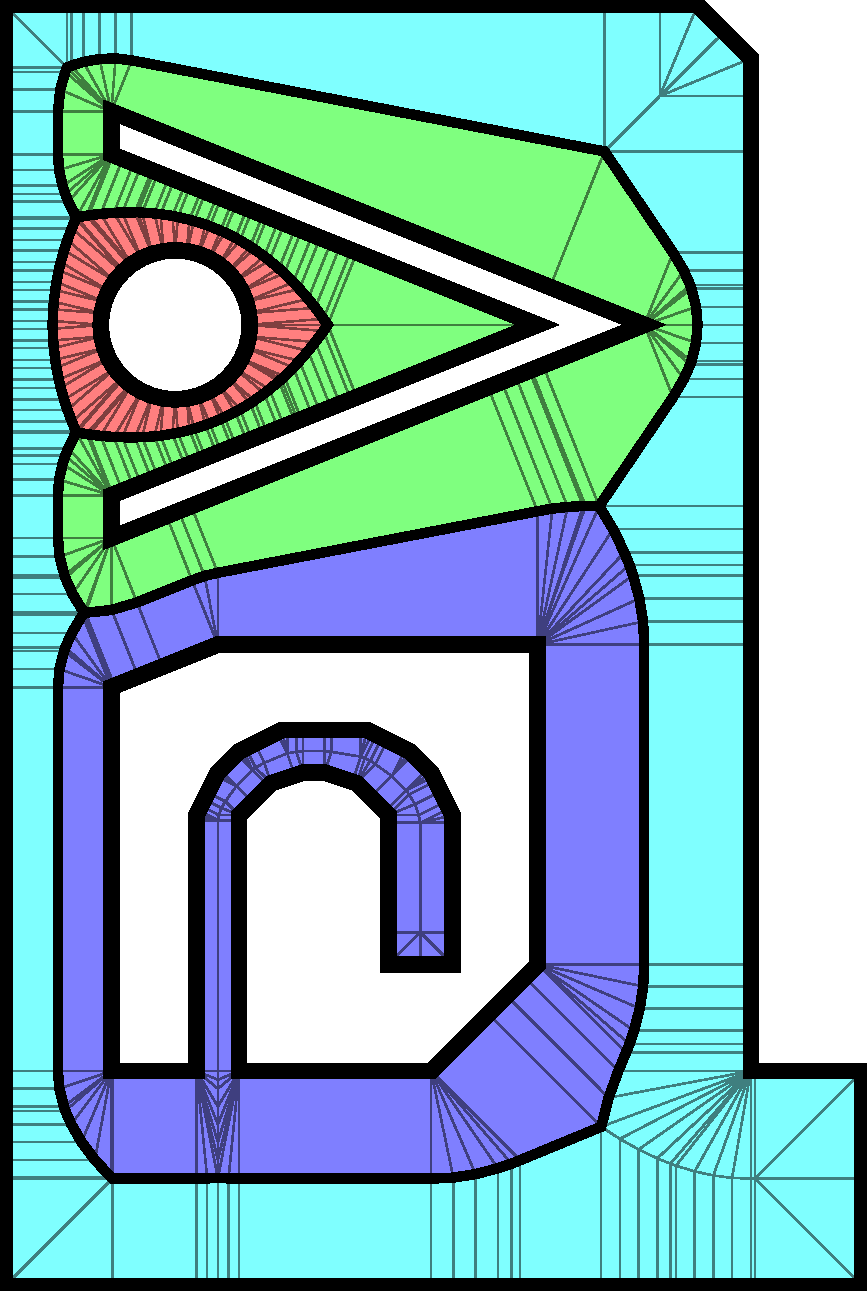
\includegraphics[width=\figheight,rotate=90]{sources/method/domains.pdf}
\caption{Polygon domains}\label{shape_decomposition_domains}
\end{subfigure}
\begin{subfigure}{.45\columnwidth}\centering
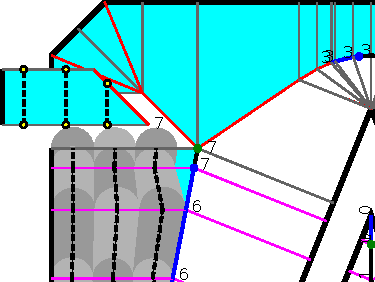
\includegraphics[height=\figheight]{sources/method/segment_generation.pdf}
\caption{Extrusion segment chaining}\label{shape_decomposition_domains}
\end{subfigure}
\caption{
Generating toolpaths on a part of the test outline shape by chaining together extrusion segments along each polygon domain.
Each edge is assigned toolpath sites (yellow) which are connected together as shown in the singled out trapezoid.
By following the trapezoids along the domain (cyan) of a single outline polygon,
the extrusion segments can efficiently be connected into existing polyline toolpaths (light and dark gray).
}
\label{segment_generation}
\end{figure}


Around the transition locations and around nodes with odd bead count and more than two marked edges attached there will be intersections in the toolpaths.
Such intersections cause overfill because the nozzle passes the location multiple times.
We deal with this special case by forcing a new polyline when traversing the trapezoids, and in the final polyline connection step we greadily connect the first two polylines ending in the same location and retreat all other polylines ending in that same location in order to prevent the overfill.
In order to retreat a polyline which ends in a site $S$ we remove part of the polyline paths up to the intersection by a distance of $w^S d_\text{max}^\text{intersection}$, where $d_\text{max}^\text{intersection}$ is some ration between $0$ and $1$.
This ratio effectively deals with the balance between overfill and underfill generated at that location after the retreat has been applied.
See \cref{polyline_reduction}.


\begin{figure}
\centering
\setlength{\figwidth}{.35\columnwidth}
\begin{subfigure}{0.45\columnwidth}\centering
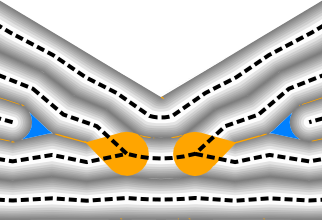
\includegraphics[width=\figwidth,frame]{sources/method/polyline_reduction_before}
\caption{No reduction}
\end{subfigure}
\begin{subfigure}{0.45\columnwidth}\centering
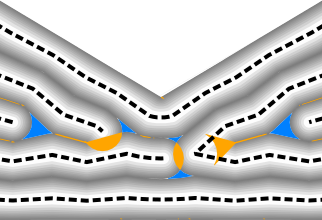
\includegraphics[width=\figwidth,frame]{sources/method/polyline_reduction_after}
\caption{Reduction}
\end{subfigure}
\caption{
Reducing polyline toolpaths away from intersections in order to prevent overfill.
Toolpath locations in black, underfill in azure and overfill in orange.
}
\label{polyline_reduction}
\end{figure}





























































\section{Results and discussion}

We evaluate the proposed framework and the various beading schemes on a set of different types of 3D models, ranging over various applications and various types of geometry. 
The data set is described in Appendix~\ref{dataset}.
We sliced all models in the data set and selected 300 random slices for analysis.
Toolpaths of these 300 outline shapes are generated using the uniform technique as implemented by Clipper~\cite{johnson2014clipper} -- a state-of-the-art polygon offset library, and by our framework using four beading schemes, i.e. the constant bead count scheme with a bead count of $C=4$, the centered, the evenly distributed, and the inward distributed beading scheme using $N=3$, all with a preferred bead widths of $w^* = \SI{0.4}{\milli\meter}$. The tests were performed on a desktop PC equipped with an Intel Core i7-7500U CPU @ \SI{2.70}{\giga\hertz} (a single core is used) and \SI{16.3}{\giga\byte} memory.





\subsection{Computational results}


\subsubsection{Accuracy}
We first evaluate the accuracy of different beading schemes in terms of the relative amount of the overfill and underfill. 
\begin{wrapfigure}{r}{.3\columnwidth}
\centering

\includegraphics[width=.25\columnwidth]{sources-validation-visualization-principle-rounded-excluded-single.pdf}
\caption{
Extrusion segments coverage.
The hole at the end will be filled by the next extrusion segment.
}
\label{segment_visualization_simple}
\end{wrapfigure}
We construct the over- and underfill area by comparing the shapes covered by each extrusion move (\cref{segment_visualization_simple}) with each other and with the total shape of the boundary polygons. (For implementation details see Appendix~\ref{accuracy_calculation}.)
This results in polygonal shapes such as visualized in the top half of \cref{visualized_accuracy}:
there are orange shapes where the beads overlap and azure shapes in the voids in between the beads.


We compare the total area in \si{\milli\meter\squared} of these overfill and underfill shapes to the total area of the boundary for each sample in the data set
and report the average percentages in see \cref{over_underfill}.
The inward distributed scheme has a calculated overfill of \SI{0.24}{\percent} and an underfill of \SI{0.17}{\percent}.
This is lower compared to the uniform scheme, which results in \SI{1.2}{\percent} overfill and \SI{1.7}{\percent} underfill in the data set.

\begin{figure*}
\centering
\setlength{\figwidth}{0.19\textwidth}
\setlength{\figheight}{0.283\textwidth}
\begin{subfigure}{\figwidth}\centering
\includegraphics[height=\figheight]{sources-validation-gMAT-example-TEST-naive-accuracy.png}
\includegraphics[height=\figheight]{sources-validation-gMAT-example-TEST-naive-widths.png}
\caption{Uniform}\label{TEST_naive_accuracy}
\end{subfigure}
%\begin{subfigure}{\figwidth}\centering
%\includegraphics[height=\figheight]{sources-validation-gMAT-example-TEST-SingleBead-accuracy.png}
%\includegraphics[height=\figheight]{sources-validation-gMAT-example-TEST-SingleBead-widths.png}
%\caption{Single}\label{TEST_SingleBead_accuracy}
%\end{subfigure}
\begin{subfigure}{\figwidth}\centering
\includegraphics[height=\figheight]{sources-validation-gMAT-example-TEST-Constant-accuracy.png}
\includegraphics[height=\figheight]{sources-validation-gMAT-example-TEST-Constant-widths.png}
\caption{Constant}\label{TEST_Constant_accuracy}
\end{subfigure}
\begin{subfigure}{\figwidth}\centering
\includegraphics[height=\figheight]{sources-validation-gMAT-example-TEST-Center-accuracy.png}
\includegraphics[height=\figheight]{sources-validation-gMAT-example-TEST-Center-widths.png}
\caption{Centered}\label{TEST_Center_accuracy}
\end{subfigure}
\begin{subfigure}{\figwidth}\centering
\includegraphics[height=\figheight]{sources-validation-gMAT-example-TEST-Distributed-accuracy.png}
\includegraphics[height=\figheight]{sources-validation-gMAT-example-TEST-Distributed-widths.png}
\caption{Distributed}\label{TEST_Distributed_accuracy}
\end{subfigure}
\begin{subfigure}{\figwidth}\centering
\includegraphics[width=\columnwidth]{sources-validation-gMAT-example-TEST-InwardDistributed-accuracy.png}
\includegraphics[width=\columnwidth]{sources-validation-gMAT-example-TEST-InwardDistributed-widths.png}
\caption{Inward}\label{TEST_InwardDistributed_accuracy}
\end{subfigure}
\begin{subfigure}{.04\columnwidth}\centering
\vspace{4.7cm}
\includegraphics[height=\figheight]{sources-validation-gMAT-example-widths-legend.pdf}
\end{subfigure}
\caption{
Visualization of the overfills and underfills (top) and the widths (bottom) for various beading schemes.
Extrusion beads in gray tones,
overfill in orange,
underfill in azure,
narrow beads in blue
and wide beads in red.
}
\label{visualized_accuracy}
\end{figure*}




\begin{figure*}
\centering
\setlength{\figheight}{0.22\textwidth}
\setlength{\figwidth}{0.31\textwidth}
\begin{subfigure}{\figwidth}\centering
\includegraphics[height=\figheight]{sources-validation-computime2.pdf}
%\includegraphics[width=\figwidth]{sources-validation-computime2.pdf}
\caption{Computation time}
\label{computime}
\end{subfigure}
\begin{subfigure}{\figwidth}\centering
\includegraphics[height=\figheight]{sources-validation-widthHistogram.pdf}
%\includegraphics[width=\figwidth]{sources-validation-widthHistogram.pdf}
\caption{Extrusion widths}
\label{widthHistogram}
\end{subfigure}
\begin{subfigure}{\figwidth}\centering
\includegraphics[height=\figheight]{sources-validation-indexedwidths2.pdf}
%\includegraphics[width=\figwidth]{sources-validation-widthHistogram.pdf}
\caption{Extrusion width per index}
\label{widthIndexedHistogram}
\end{subfigure}
\begin{subfigure}{\figwidth}\centering
\includegraphics[height=\figheight]{sources-validation-overunderfill.pdf}
%\includegraphics[width=\figwidth]{sources-validation-overunderfill.pdf}
\caption{Over- and underfill}
\label{over_underfill}
\end{subfigure}
\begin{subfigure}{\figwidth}\centering
\includegraphics[height=\figheight]{sources-validation-smoothness.pdf}
%\includegraphics[width=\figwidth]{sources-validation-smoothness.pdf}
\caption{Site angles}
\label{smoothness}
\end{subfigure}
\begin{subfigure}{\figwidth}\centering
\includegraphics[height=\figheight]{sources-validation-smoothnessNoTransition.pdf}
%\includegraphics[width=\figwidth]{sources-validation-smoothnessNoTransition.pdf}
\caption{Site angles without smoothing}
\label{smoothnessNoTransition}
\end{subfigure}


\caption{
Statistical analysis of the toolpaths from applying the uniform width technique and various beading schemes using our framework to a data set of 300 slices.
Note the use of a logarithmic scale on the Y-axes and on some of the X-axes as well.
}
\end{figure*}









\subsubsection{Uniformity}
We visualize the bead widths resulting from the different schemes in the bottom of \cref{visualized_accuracy}.
We calculated the mean and standard deviation of the bead width, sampled at \SI{1}{\micro\meter} along the toolpaths.
\cref{widthHistogram} shows the distribution of extrusion width for each scheme binned at intervals of \SI{10}{\micro\meter}.
We found that the mean width of the inward and evenly distributed schemes is close to preferred bead width of \SI{400}{\micro\meter}, while their standard deviation is lower than for the centered and constant bead count scheme. 
These results indicate that, while causing less overfill and underfill, inwards distributed and evenly distributed schemes deviate less or less often from the preferred bead width compared to the other schemes.
We compared the width uniformity of the 6 outer beads for the inward and evenly distributed schemes, the distribution of these extrusion widths is shown in \cref{widthIndexedHistogram}. 
The outer beads of the inward distributed scheme deviate less from the preferred width compared to the evenly distributed scheme.

\subsubsection{Smoothness of toolpaths}
In order to maintain a high printing speed, it is desirable that toolpaths have fewer and less sharp corners. 
We therefore measured the angle between consecutive extrusion segments generated by each scheme
and report on the occurence of each angle in \cref{smoothness}.
All schemes show a higher number of corners for smaller angles with a peak towards \SI{180}{\degree} (straight).
We observe that compared to the naive method our framework produces less acute angles which, but more obtuse angles.
The inward distributed scheme produces an order of magnitude less corners around \SI{150}{\degree}, compared to evenly distributed. 
We also investigated the effect of the transition regions on the smoothness of the toolpaths. 
\cref{smoothnessNoTransition} shows that introducing the transitions greatly reduces the number of corners around \SI{90}{\degree}. 

\subsubsection{Computational performance}
\cref{computime} plots the computation time against the vertex count of the layer for the full data set, comparing the uniform technique implemented using Clipper~\cite{johnson2014clipper} to our framework with the inward distributed scheme.
For polygonal shapes with as many as $10^4$ vertices, the computation for both approaches is less than 1 second, with our method being approximately five times that of the uniform technique.
These results could be improved upon by utilizing the locality inherent in our algorithms for parallelization on the GPU.

The computational complexity is limited by the generation of the Voronoi Diagram, which is $O(n \log n)$, where $n$ is the number of vertices in the input shape.
The other steps in our framework have a complexity of $O(m)$, where $m$ is the number of elements in the ST.
Therefore, the total running time of our algorithm is $O(n \log n)$.
Results in \cref{computime} confirm that both our framework and the uniform technique have an expected running time of approximately $5 \times 10^{-6} n \log n$ seconds.






\subsection{Printing results}
Test prints were performed on a custom FDM hardware setup, with a standard \SI{0.4}{\milli\meter} nozzle and a filament extrusion drive directly mounted on the print head.
The firmware of the printer employs \emph{linear advance} for accurately realizing adaptive deposition width:
gaining the extra pressure required to change to a wider bead is realized by 'advancing' an extra amount of filament into the physical system~\cite{tronvoll2019investigating}.
We set the preferred width to $w^* = \SI{0.6}{\milli\meter}$, to avoid fluttered printing of lines narrower than the nozzle size.
We used a layer thickness of \SI{0.2}{\milli\meter} and a movement speed of \SI{10}{\milli\meter\per\second}.

The prints are shown in \cref{prints}.
Because of inaccuracies in the deposition control system some of the prints show defects.
Such defects are less prevalent for the inward distributed beading scheme than the other schemes.
The prints which employ the uniform offsets technique show a lot of underfill, which impacts the visual quality of the print.
Moreover, in the case of the regular honeycomb there are several fully disconnected hexagons, which means the object falls apart.
The difference between the centered and the inward distributed schemes is less pronounced.
We can still see some loosely connected extrusion segments in both, which is attributable to inaccuracies in the extrusion system.
However, the middle of \cref{wedge_print} exhibits more defects in the regions where the centered scheme produces extremal bead widths.
The bottom print shows that the inward distributed beading scheme produces smoother prints with less defects.


\begin{figure}
\centering
\begin{subfigure}{\columnwidth}\centering
\setlength{\figwidth}{\columnwidth}
\includegraphics[width=\figwidth]{sources-applications-P3-print-wedge-naive-edited.png}
\includegraphics[width=\figwidth]{sources-applications-P3-print-wedge-center-edited.png}
\includegraphics[width=\figwidth]{sources-applications-P3-print-wedge-inward-edited.png}
\caption{Uniform (top), centered (mid) and inward distributed (bottom)}\label{wedge_print}
\end{subfigure}
\setlength{\figheight}{.38\columnwidth}
\setlength{\figheightTwo}{.47\columnwidth}
\setlength{\figwidth}{0.32\columnwidth}
\begin{subfigure}{\figwidth}\centering
%\includegraphics[height=\figheightTwo]{sources-applications-gMAT-naive.png}
\includegraphics[height=\figheight]{sources-applications-P3-print-hex-naive-edited.png}
\includegraphics[width=\figwidth]{sources-applications-P3-print-UM-naive-edited.png}
\caption{Uniform}\label{print_naive}
\end{subfigure}
\begin{subfigure}{\figwidth}\centering
%\includegraphics[height=\figheightTwo]{sources-applications-gMAT-center.png}
\includegraphics[height=\figheight]{sources-applications-P3-print-hex-center-edited.png}
\includegraphics[width=\figwidth]{sources-applications-P3-print-UM-center-edited.png}
\caption{Centered}\label{print_center}
\end{subfigure}
\begin{subfigure}{\figwidth}\centering
%\includegraphics[height=\figheightTwo]{sources-applications-gMAT-inward.png}
\includegraphics[height=\figheight]{sources-applications-P3-print-hex-inward-edited.png}
\includegraphics[width=\figwidth]{sources-applications-P3-print-UM-inward-edited.png}
\caption{Inward distributed}\label{print_inward}
\end{subfigure}
\caption{
Test shapes printed using the uniform scheme, centered scheme and the inward distributed scheme.
The uniform technique produces distinct underfill areas.
The centered scheme shows some defects due to inaccurate control of extremal deposition widths.
The inward distributed scheme produces the least defects.
}
\label{prints}
\end{figure}


\iffalse
\todo{Maybe test the following qualities:}
\begin{itemize}
\item visual consistency of flat top skin surface
\item graphs of tensile tests on thin walled object
\end{itemize}
\fi










%We therefore visualize include a semi-circle with a diameter equal to the starting width in the one end, and exclude it at the other end, because it will be included in the next extrusion segment.




\section{Validation}
Print objects and show qualities:
\begin{itemize}
\item visual consistency of flat top skin surface
\item visual gradual transparency changes
\item graphs of tensile tests on thin walled object
\end{itemize}













\subsection{Applications}
Toolpath with varying width is particularly meaningful for narrow parts, since there the negative effect of under- and overfill is more pronounced than in wide parts.
In extreme cases, thin features will not be filled at all.
Therefore, our framework, while working for wide parts as well, shows most of its potential for objects which contain thin parts.

\Cref{applications_overview} collectively shows the application of the proposed inward distributed scheme for various types of 3D model, including both thin parts (architectural models, casings, embossed text, gears and microstructures) and wide parts (\cref{applications_case}) and organic shapes (\cref{applications_statue})).

For architectural models and casings, preventing over- and underfill is expected to make them stronger. 
For embossed text, preventing underfill reduces the various holes in the top surfaces, which is detrimental to the visual quality of those top surfaces.
For gears and similar mechanical parts that are designed with finite element analysis, the less variation in extrusion widths is closer to the assumptions under fast analysis (e.g. using homogenization~\cite{Liu2016CAD}).

Of particular interest are microstructures that could be uniquely fabricated by 3D printing.
For example, topology optimized bone-like structures~\cite{wu2017infill} contain filaments of varying thickness that follow a varying stress direction (\cref{applications_bone}).
An angled Gyroid structure with uniform thickness also results in outline shapes with varying width (\cref{applications_gyroid}). 
These structures are accurately densely filled using our framework.
Another class of microstructures consists of parameterized patterns with varying thickness to achieve functional gradation.
\Cref{applications_hex} shows the contour-parallel toolpath with varying width of a hexagonal grid neatly switches between different bead counts over the volume, preventing the jagged moves a direction-parallel toolpath would create for such a case~\cite{bates2018compressive}.


\begin{figure*}
\centering
\setlength{\figwidth}{0.099\textwidth}
\setlength{\figheight}{0.099\textwidth}
\begin{subfigure}{\textwidth}\centering
\censorbox{
\includegraphics[width=\textwidth]{sources-applications-combined-small-dilated-circled.pdf}
}
%\caption{Overview}\label{applications_overview}
\end{subfigure}
\begin{subfigure}[t]{\figwidth}\centering
\includegraphics[height=\figheight]{sources-applications-house.png}
\caption{House}\label{applications_house}
\end{subfigure}
\begin{subfigure}[t]{\figwidth}\centering
\includegraphics[height=\figheight]{sources-applications-pocket-operator-case.png}
\caption{Case}\label{applications_case}
\end{subfigure}
\begin{subfigure}[t]{\figwidth}\centering
\includegraphics[height=\figheight]{sources-applications-david.png}
\caption{Statue}\label{applications_statue}
\end{subfigure}
\begin{subfigure}[t]{\figwidth}\centering
\censorbox{
\includegraphics[height=\figheight]{sources-applications-tud-logo.png}
}
\caption{\censor{TUD}}\label{applications_tud}
\end{subfigure}
\begin{subfigure}[t]{\figwidth}\centering
\censorbox{
\includegraphics[height=\figheight]{sources-applications-ultimaker-logo.png}
}
\caption{\censor{UM}}\label{applications_um}
\end{subfigure}
\begin{subfigure}[t]{\figwidth}\centering
\includegraphics[height=\figheight]{sources-applications-pinion-gear-motor.png}
\caption{Gear}\label{applications_gear}
\end{subfigure}
\begin{subfigure}[t]{\figwidth}\centering
\includegraphics[height=\figheight]{sources-applications-topopt-bone.png}
\caption{Bone}\label{applications_bone}
\end{subfigure}
\begin{subfigure}[t]{\figwidth}\centering
\includegraphics[height=\figheight]{sources-applications-gyroid.png}
\caption{Gyroid}\label{applications_gyroid}
\end{subfigure}
\begin{subfigure}[t]{\figwidth}\centering
\includegraphics[height=\figheight]{sources-applications-hex-grid.png}
\caption{Hex}\label{applications_hex}
\end{subfigure}
\begin{subfigure}[t]{.3\figwidth}
\includegraphics[height=\figheight]{sources-validation-widths-legend-small.pdf}
\end{subfigure}
\caption{
Visualization of the widths for the output toolpaths of the inward distributed beading scheme {($N=3$) }applied to various example application objects.
From left to right and top to bottom: a house, a case for electronics, a statue, two common logos, a gear, a topologically optimized bone structure, a tilted homogeneous gyroid structure and a heterogeneous thickness hexagonal grid.
}
\label{applications_overview}
\end{figure*}






\section{Conclusion}
In this paper we have introduced a framework for computing contour-parallel toolpaths employing adaptive bead width in order to minimize underfill and overfill areas\revise{.}{,
we introduced beading schemes which improve on the state of the art
and we have introduced a back pressure compensation method for accurate fabrication of adaptive width.
}

Our framework is flexible, demonstrated by the several beading schemes which emulate existing techniques.
The computation times of our framework are on par with the state-of-the-art library for performing offsets of non-adaptive bead width.
Our framework is stable: small local changes in the outline shape cause only small changes in the toolpath.

\revise{We presented}{Compared to the state of the art,} the inward distributed beading scheme
\revise{It}{} reduces the amount of beads with a width deviating extremely from the preferred bead width \revise{}{by changing the width of several beads near the center instead of only the center-most bead}.
\revise{, and thus it is}{It is therefore} expected to limit the impact of varying the bead width in terms of production accuracy and homogeneity of material properties,
which in turn is helpful to efficiently simulate an FDM manufactured part.
\revise{
Furthermore, by distributing the deviation in bead width over several beads near the center of the shape, the outer toolpath is affected less by the deviation, meaning that the dimensional accuracy of the shape of the outline contour is affected less by inaccuracies in the mechanical control system which realizes adaptive bead width.
}{}

The proposed beading scheme greatly improves the process planning for parts with thin contours, which often occur for example in architectural models, prototypes for casings or microstructures.
Meanwhile it leaves most of the toolpaths the same as the uniform width technique in large features, meaning that existing studies which relate process parameters with mechanical properties of the print are still applicable.
\revise{}{Compared to the naive approach of constant width toolpaths our beading scheme is expected to improve the stiffness, dimensional accuracy and visual qualities of the manufactured model.}
\revise{}{It is expected that as distributed beading schemes are implemented in commercial software packages and bead width variation control become commonplace, the practice of design for additive manufacturing can disregards some of the nozzle size considerations.}

\medskip
\revise{}{The presented framework is open source available at \\ \url{github.com/Ultimaker/libArachne}}


\revise{
\subsection{Future work}
The work presented here is evaluated mostly on a computational level, because the effectiveness of a mechanical system to accurately print an adaptive bead width interferes with the physical validation of our techniques.
Future research could be devoted to optimizing the distribution scheme to a specific hardware setup.
An accurate model of manufacturability, print speed and dimensional accuracy would be valuable to fine-tune the beading scheme.
% If we can assign a loss function to several aspects (e.g. manufacturability, print speed, dimensional accuracy) of a toolpath we could deduce the optimal beading scheme.
}{}

\revise{
Our framework uses the skeleton to determine toolpaths based on the local feature size.
Another direction of future research could be devoted to incorporating other information, e.g. properties of the outline such as curvature or visibility, non-local features such as the size of nearby outline features, toolpaths of the previous layer, or voluminal constraints (e.g. for functionally graded materials).
% Furthermore we could also take into account volumetric considerations such as the toolpathing of the previous layer or volume constraint defined by a functionally graded material.
}{}
% Taking a broader perspective we note that the skeletonization decomposes a shape into trapezoids and these trapezoids are decomposed into quads by the toolpath segments which we generate for it.
% It would be interesting to see if similar technique can be used to generate quad dominant meshings for finite element analysis.


\section*{References}
\bibliography{99_mybib}

\end{document}
